% Sample file for the use of compsoft style file.
%
\documentclass[S,R,E]{article/compsoft}
% Preamble
%
% 「コンピュータソフトウェア」誌に掲載される論文の場合,次で
% 巻数,号数,開始ページ,終了ページを指定する.
\volNoPp{0}{0}{0}{0}

% ワークショップによる推薦論文の場合,ワークショップ名を指定する.
% \suisen{ワークショップ名}

% 特集の場合,特集のタイトルを与える.
% \tokushu{特集のタイトル}

% 大会論文の場合,¥taikai で開催年を指定する.ここで指定した年から
% 大会の回数は計算される.
% \taikai{2009}

% ここに,使用するパッケージを列挙する.
%\usepackage[dvips]{graphics}
\usepackage[dvipdfmx]{graphicx}
\usepackage{amssymb}
\usepackage{float}
\usepackage{enumerate,cite,url}
\usepackage{listings,jlisting}
\lstset{%
    language={c},%
    basicstyle={\small},%
    identifierstyle={\small},%
    commentstyle={\footnotesize\itshape},%
    keywordstyle={\small},%\bfseries},%
    ndkeywordstyle={\small},%
    stringstyle={\small\it},
    frame={tb},
    breaklines=true,
    columns=[l]{fullflexible},%
    numbers=left,%
    xrightmargin=0zw,%
    xleftmargin=3zw,%
    numberstyle={\scriptsize},%
    stepnumber=1,
    numbersep=1zw,%
    lineskip=-0.5ex%
}

% ユーザが定義したマクロなどはここに置く.ただし学会誌のスタイルの
% 再定義は原則として避けること.

\begin{document}

% 論文のタイトル
\title{Component-Based Framework of Lightweight Ruby for Efficient Embedded Software Development}

% 著者
% 和文論文の場合,姓と名の間には半角スペースを入れ,
% 複数の著者の間は全角スペースで区切る
%
\author{Takuro Yamamoto Hiroshi Oyama Takuya Azumi}
%
% ここにタイトル英訳 (英文の場合は和訳) を書く.
%
\ejtitle{軽量Rubyを用いた効率的な組込みソフトウェア開発コンポーネントベースフレームワーク}
%
% ここに著者英文表記 (英文の場合は和文表記) および
% 所属 (和文および英文) を書く.
% 複数著者の所属はまとめてよい.
%
\shozoku{山本 拓朗, 安積 卓也}{大阪大学大学院基礎工学研究科}%
{Graduate School of Engineering Science, Osaka University}
\shozoku{大山 博司}{オークマ株式会社}%
{OKUMA Corporation}

%
% 出典情報は \shutten とすれば出力される.
\shutten
%
% 受付年月日,記事カテゴリなどは自動的に生成される.
\uketsuke{0000}{00}{00}
%
% その他,脚注に入れるものがあれば,¥note に記述する.
%\note{脚注に入れる内容}


%
% 和文アブストラクト
% \Jabstract{%
% 近年,組込みシステムは複雑化・大規模化しているため,ソフトウェアの生産性が問題になっている.
% 組込みソフトウェア開発の生産性の向上を目的として,mruby(軽量Ruby)を適用させたコンポーネントベース開発が可能なフレームワークであるmruby on TECSを提案してきた.
% 現状のmruby on TECSでは,プラットフォームにmrubyバイトコードを組み込んでいるため,mrubyプログラムを修正する度にコンパイル・リンクし直す必要がある.
% さらに,マルチVMを提供しているが,複数のmrubyプログラムを効率良く並行動作させるには開発者がリアルタイムOSの機能を熟知している必要がある.
% 本研究では,mruby on TECSの拡張として,mrubyアプリケーションのバイトコードをBluetoothで転送することで開発効率を向上させる.
% さらに,複数のmrubyプログラムを協調動作できるフレームワークを提案する.
% }
%
% 英文アブストラクト(本サンプルの原論文にはなし)
\Eabstract{
The complexity and scale of embedded software have increased.
To improve the productivity, the mruby on TOPPERS embedded component system (TECS) framework, which employs a scripting language (i.e., lightweight Ruby) and supports component-based development, has been proposed.
In the current mruby on TECS framework, mruby programs must be compiled and linked every time they are modified, because mruby bytecode are incorporated in the platform.
Moreover, while the framework supports multiple virtual machines (VMs), developers must be familiar with the functions of real-time operating systems to effectively execute multiple mruby programs concurrently or in parallel.
This paper proposed an extended mruby on TECS framework that improves development efficiency more than the current framework.
We implemented a Bluetooth loader receives an mruby bytecode, and a RiteVM scheduler simplifies multitasking.
Synchronization of initializing multiple tasks is also implemented using an Eventflag.
Experimental results demonstrate the advantages of the proposed framework.
}
%
\maketitle

%%%%%%%%%%%本文%%%%%%%%%%%%%%%%%%%%%%%%%%%%

\section{Introduction}
Currently, embedded systems, e.g., Internet of Things applications, must demonstrate high quality and high performance.
This requirement has led to an increase in their complexity and scale; moreover, these systems need to have low production costs and short development cycles.

Complex and large-scale software systems can be developed efficiently by using component-based techniques \cite{par:Crnkovic}, \cite{par:CBD}.
Component-Based Development (CBD) is a design technique that can be applied to reusable software development.
% Complex and large scale software systems can be developed efficiently using component-based techniques.
% That is because software componentization provides high-reusability.
Verification of component-based systems has been extensively researched \cite{par:Blaming}, \cite{par:Verification}.
Individual component diagrams enable the visualization of an entire system.
%It also visualize the entire system due to component diagrams, and makes a system flexible in extensions and specification changes.
In addition, component-based systems are flexible with regard to extensibility and specification changes.
The TOPPERS embedded component system (TECS) \cite{par:TECS}, AUTOSAR \cite{url:AUTOSAR}, and SaveCCM \cite{par:SAVEapproach} are typical CBD tools for embedded systems.

In addition, scripting languages, such as Ruby, JavaScript, Perl, Python, and Lua, offer efficient approaches to software development.
Currently, most software are programmed in C language.
However, development in C language results in large code size, incurs high costs, and requires significant development time.
In contrast, the use of scripting languages improves the efficiency of software engineering and can shorten the development period because it is relatively easy to reuse scripts. 
% script languages have high-productivity from their usability.
% Ruby, JavaScript, Perl, Python, and Lua are well-known as representative script languages.

For embedded systems, real-time properties, such as estimation of worst-case execution time, are very important.
Although scripting languages are easy to use and read, their execution requires more time than that required by the codes written in C.
Therefore, applying scripting languages to embedded systems is difficult.

To address the above limitation, ``mruby on TECS,'' a component-based framework for running script programs, has been proposed \cite{par:mrubyonTECS}.
This framework integrates two technologies, i.e., mruby, which is a lightweight implementation of Ruby for embedded systems \cite{par:mruby}, \cite{url:mruby}, and TECS, which is a component-based framework for embedded systems \cite{par:TECS}, \cite{url:TOPPERS}.
% mruby on TECS supports to effectively run mruby script language on embedded systems.
% mruby on TECS also makes execution time 100 times faster than that of mruby.

%This paper proposes two additional features of mruby on TECS, Bluetooth loader for mruby bytecode and RiteVM scheduler.
Even though execution times of mruby on TECS are 100 times faster than those of mruby, it is not particularly efficient, at present, and imposes a heavy burden on developers.
Moreover, mruby on TECS only supports a storage/ROM device for loading mruby programs.
Consequently, if mruby programs are modified, a secure digital (SD) card must be inserted and removed repeatedly or ROM must be rewritten; moreover, developers need to restart real-time operating systems (RTOSs) on the target device.
In addition, although mruby on TECS can support multiple virtual machines (multi-VMs), executing multiple tasks requires the developers to call the OS function.

This paper proposes an extended framework of mruby on TECS that comprises a Bluetooth loader for mruby bytecode and a RiteVM scheduler for fairly executing mruby programs.
To improve development efficiency, in the proposed framework, developers need to implement the platform on a storage device only once at the beginning and can transfer mruby application programs from a host to a target device using the Bluetooth loader.
Note that RiteVM is the Ruby VM specifically designed for embedded systems.
The RiteVM scheduler manages the execution of multiple RiteVMs and allows developers to program multitasking more easily than the current version of mruby on TECS.

{\bf Contributions}: The proposed framework provides the following contributions:
\begin{enumerate}
\item {\bf Improved software development efficiency.}
Developers do not need to rewrite a storage/ROM device and restart an RTOS.
The Bluetooth loader supports continuous loading, which reduces Bluetooth set-up time (i.e., pairing).
\item {\bf Execution of multiple mruby programs concurrently or in parallel.}
Developers can implement multiple tasks without RTOS knowledge because the RiteVM scheduler switches tasks cyclically.
\item {\bf Synchronized execution of multiple RiteVM tasks.}
The proposed framework synchronizes multiple RiteVM tasks (i.e., mruby applications).
\item {\bf Benefits of CBD:}
The paper focuses on the benefits of CBD and provides specific examples.
\end{enumerate}

{\bf Organization}: The reminder of this paper is organized as follows.
Section \ref{sec:Background} introduces the basic technologies, i.e., mruby, TECS, and mruby on TECS.
Section \ref{sec:Design and Implementation} describes the design and implementation of the proposed framework.
Section \ref{sec:Evaluation} evaluates the proposed framework.
Related work is discussed in Section \ref{sec:Related work}.
In Section \ref{sec:Results}, the utilization results are reported.
Conclusions and suggestions for future work are presented in Section \ref{sec:Conclusion}.


\begin{figure}[t]
    \centering
    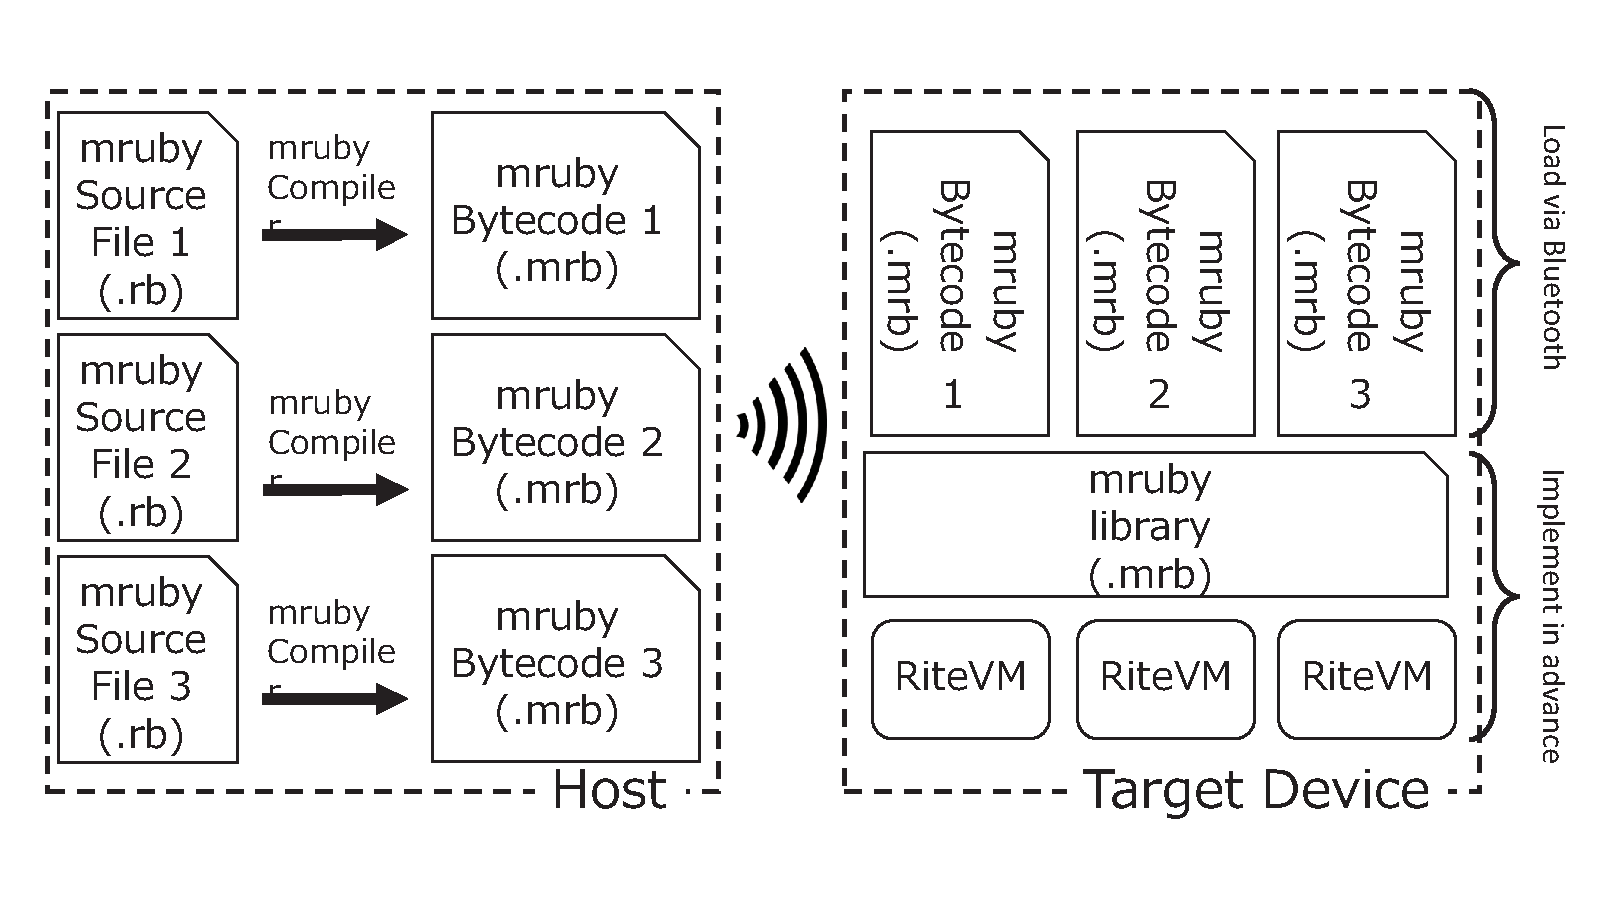
\includegraphics[width=6.5cm,clip]{figure/proposed.eps}
    \caption{System model of the proposed framework}
    \label{fig:proposed}
\end{figure}

\section{Background}
\label{sec:Background}
Fig.\ref{fig:proposed} shows the system model of the proposed framework.
Note that the RiteVMs and the mruby library are assumed to be prepared in advance.
Bytecodes are transferred from the host to the target device via Bluetooth, and each RiteVM is allocated a bytecode.
Bytecodes transferred from the host via Bluetooth can run in multitask.

The proposed framework is an extension of mruby on TECS framework \cite{par:mrubyonTECS}, and utilizes two technologies: mruby and TECS.
In this section, mruby (\ref{sec:mruby}), TECS (\ref{sec:TECS}), and mruby on TECS framework (\ref{sec:mruby on TECS}) are described.

\subsection{mruby}
\label{sec:mruby}
mruby is a light-weight implementation of the Ruby programming language complying to part of the ISO standard.
Ruby is an object-oriented scripting language \cite{url:Ruby} with classes and methods, exceptions, and garbage collection functions.
It is easy to use and read due to its simple grammar and Ruby requires fewer lines of code than C.
Ruby improves the productivity of software development due to its simple grammar and object-oriented functions.

mruby, which retains the usability and readability of Ruby, requires fewer resources, and thus, is suitable for embedded systems.
In addition, mruby includes a VM mechanism, and thus, mruby programs can run on any operating system as long as a VM is implemented.
The mruby/RiteVM mechanism is shown in Fig.\ref{fig:mruby}.
The mruby compiler translates an mruby code into a bytecode, which can be interpreted by a RiteVM; thus, mruby programs can be executed on any target device with a RiteVM.
\begin{figure}[t]
    \centering
    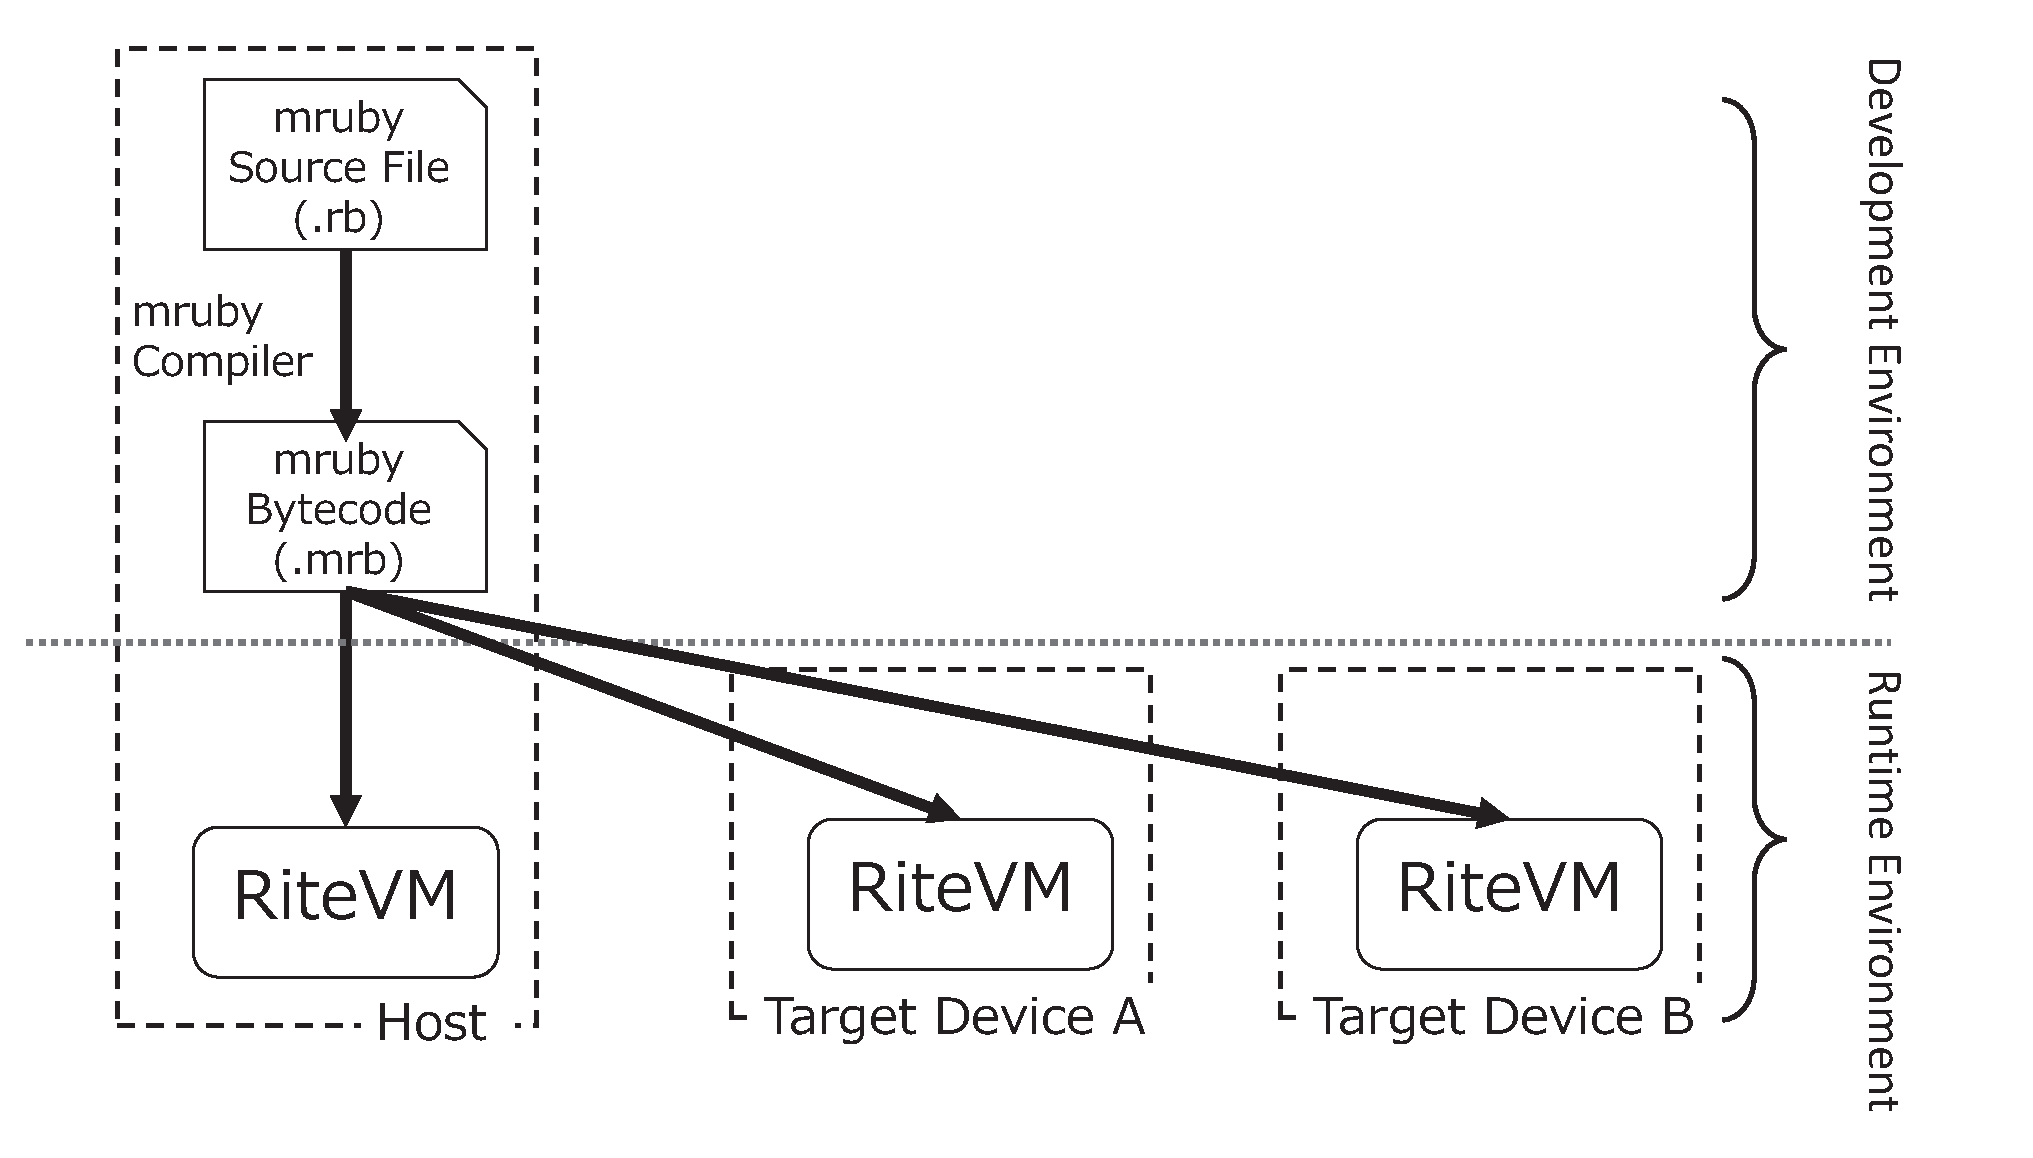
\includegraphics[width=6.5cm,clip]{figure/mruby.eps}
    \caption{mruby/RiteVM mechanism}
    \label{fig:mruby}
\end{figure}

\subsection{TECS}
\label{sec:TECS}
TECS is a component system suitable for embedded systems.
TECS can increase productivity and reduce development costs due to improved reusability of software components.
TECS also provides component diagrams, which help developers visualize the overall structure of a system.

In TECS, component deployment and composition are performed statically.
Consequently, connecting components does not incur significant overhead and memory requirements can be reduced.
TECS can be implemented in C, and demonstrates various feature such as source level portability and fine-grained components.

\begin{figure}[t]
    \centering
    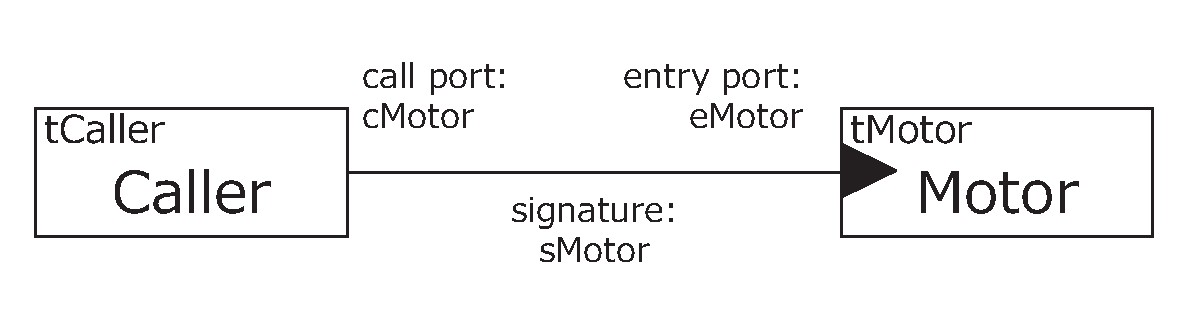
\includegraphics[width=6.5cm,clip]{figure/component_diagram.eps}
    \caption{Component Diagram}
    \label{fig:component}
\end{figure}

\subsubsection{Component Model}
Fig.\ref{fig:component} shows a component diagram.
A {\it cell}, which is an instance of a component in TECS, consists of {\it entry} ports, {\it call} ports, attributes and internal variables.
An {\it entry} port is an interface that provides functions to other {\it cell}s, and a {\it call} port is an interface that enables the use of other {\it cell}'s functions.
A {\it cell} has one or more {\it entry} ports and {\it call} ports.
{\it Cell} functions are implemented in C.

The type of {\it entry}/{\it call} port is defined by a {\it signature}, which is a set of functions.
A {\it signature} is the interface definition of a {\it cell}.
The {\it cell}'s  {\it call} port can be connected to the {\it entry} port of another {\it cell} by the same {\it signature}.
Here, {\it celltype} defines one or more {\it call}/{\it entry} ports, attributes, and internal variables of a {\it cell}.


\subsubsection{Component Description}
In TECS, components are described by {\it signature}, {\it celltype}, and build written in component description language (CDL).
% TECS code is written in CDL (component description language) file.
These components are described as follows.

\begin{description}
    \item[{\bf Signature Description}]\mbox{}\\
        The {\it signature} defines a {\it cell} interface.
        The {\it signature} name follows the keyword {\it signature} and takes the prefix ``s'' e.g., sMotor (Fig.\ref{signature}).
        In TECS, to clarify the function of an interface, specifiers such as [in] and [out] are used, which represent input and output, respectively.
\begin{figure}[t]
\centering
\begin{lstlisting}
signature sMotor {
    int32_t getCounts( void );
    ER resetCounts( void );
    ER setPower( [in]int power );
    ER stop( [in] bool_t brake );
    ER rotate( [in] int degrees,
               [in] uint32_t speed_abs,
                [in] bool_t blocking );
    void initializePort( [in]int32_t type );
};
\end{lstlisting}
\caption{Signature Description}
\label{signature}
\end{figure}
    \item[{\bf Celltype Description}]\mbox{}\\
        The {\it celltype} defines {\it entry} ports, {\it call} ports, attributes, and variables.
        A {\it celltype} name with the prefix ``t'' follows the keyword {\it celltype}, e.g., tCaller (Fig.\ref{celltype}).
        To define {\it entry} ports, a {\it signature}, e.g., sMotor, and an {\it entry} port name, e.g., eMotor, follow the keyword {\it entry}.
        {\it Call} ports are defined similarly.
        Attributes and variables follow the keywords {\it attr} and {\it var}, respectively.
\begin{figure}[t]
\centering
\begin{lstlisting}
celltype tCaller {
    call sMotor cMotor;
};
celltype tMotor {
    entry sMotor eMotor;
    attr {
        int32_t port;
    };
    var {
        int32_t currentSpeed = 0;
    };
};
\end{lstlisting}
\caption{Celltype Description}
\label{celltype}
\end{figure}
    \item[{\bf Build Description}]\mbox{}\\
        The build description is used to instantiate and connect {\it cell}s.
        Fig.\ref{build} shows an example of a build description.
        A {\it celltype} name and {\it cell} name, e.g., tMotor and Motor, respectively, follow the keyword {\it cell}.
        To compose {\it cell}s, a {\it call} port, {\it cell}'s name, and an {\it entry} port are described in that order.
        In Fig.\ref{build}, {\it entry} port eMotor in {\it cell} Motor is connected to {\it call} port cMotor in {\it cell} Caller.
        {\it C\_EXP} calls macros defined in C files.

\begin{figure}[t]
\centering
\begin{lstlisting}
cell tMotor Motor {
    port = C_EXP("PORT_A");
};
cell tCaller Caller {
    cMotor = Motor.eMotor;
};
\end{lstlisting}
\caption{Build Description}
\label{build}
\end{figure}

\end{description}

\subsection{mruby on TECS}
\label{sec:mruby on TECS}
mruby on TECS is a component-based framework for running an mruby script language on embedded systems.
This framework integrates two technologies, mruby and TECS, and enables to develop embedded software using a script language without slowing down the execution time. 

\subsubsection{System Model of mruby on TECS}
The present mruby on TECS system model is shown in Fig.\ref{fig:mrubyontecs}.
Each mruby program, which is a bytecode, runs on its own RiteVM as a componentized task of an RTOS.
TECS components support various embedded drivers such as motor and sensor drivers.

An mruby-TECS bridge provides native libraries for mruby and can call a native program (e.g., C legacy code) from an mruby program.
The mruby-TECS bridge also provides TECS components for receiving the invocation from an mruby program.
% The mruby-TECS bridge is described in more detail bellow.

In this paper, TOPPERS/HRP2 \cite{url:HRP2}, \cite{par:hr-tecs} is the target RTOS and is based on $\mu$ITRON \cite{par:microITRON} with memory protection.
However, mruby on TECS does not depend on the RTOS because TECS supports not only TOPPERS/HRP2 but also the other RTOSs such as OSEK \cite{par:OSEK} and TOPPERS/ASP \cite{par:ASP}, \cite{url:ASP}.

\begin{figure}[t]
    \centering
    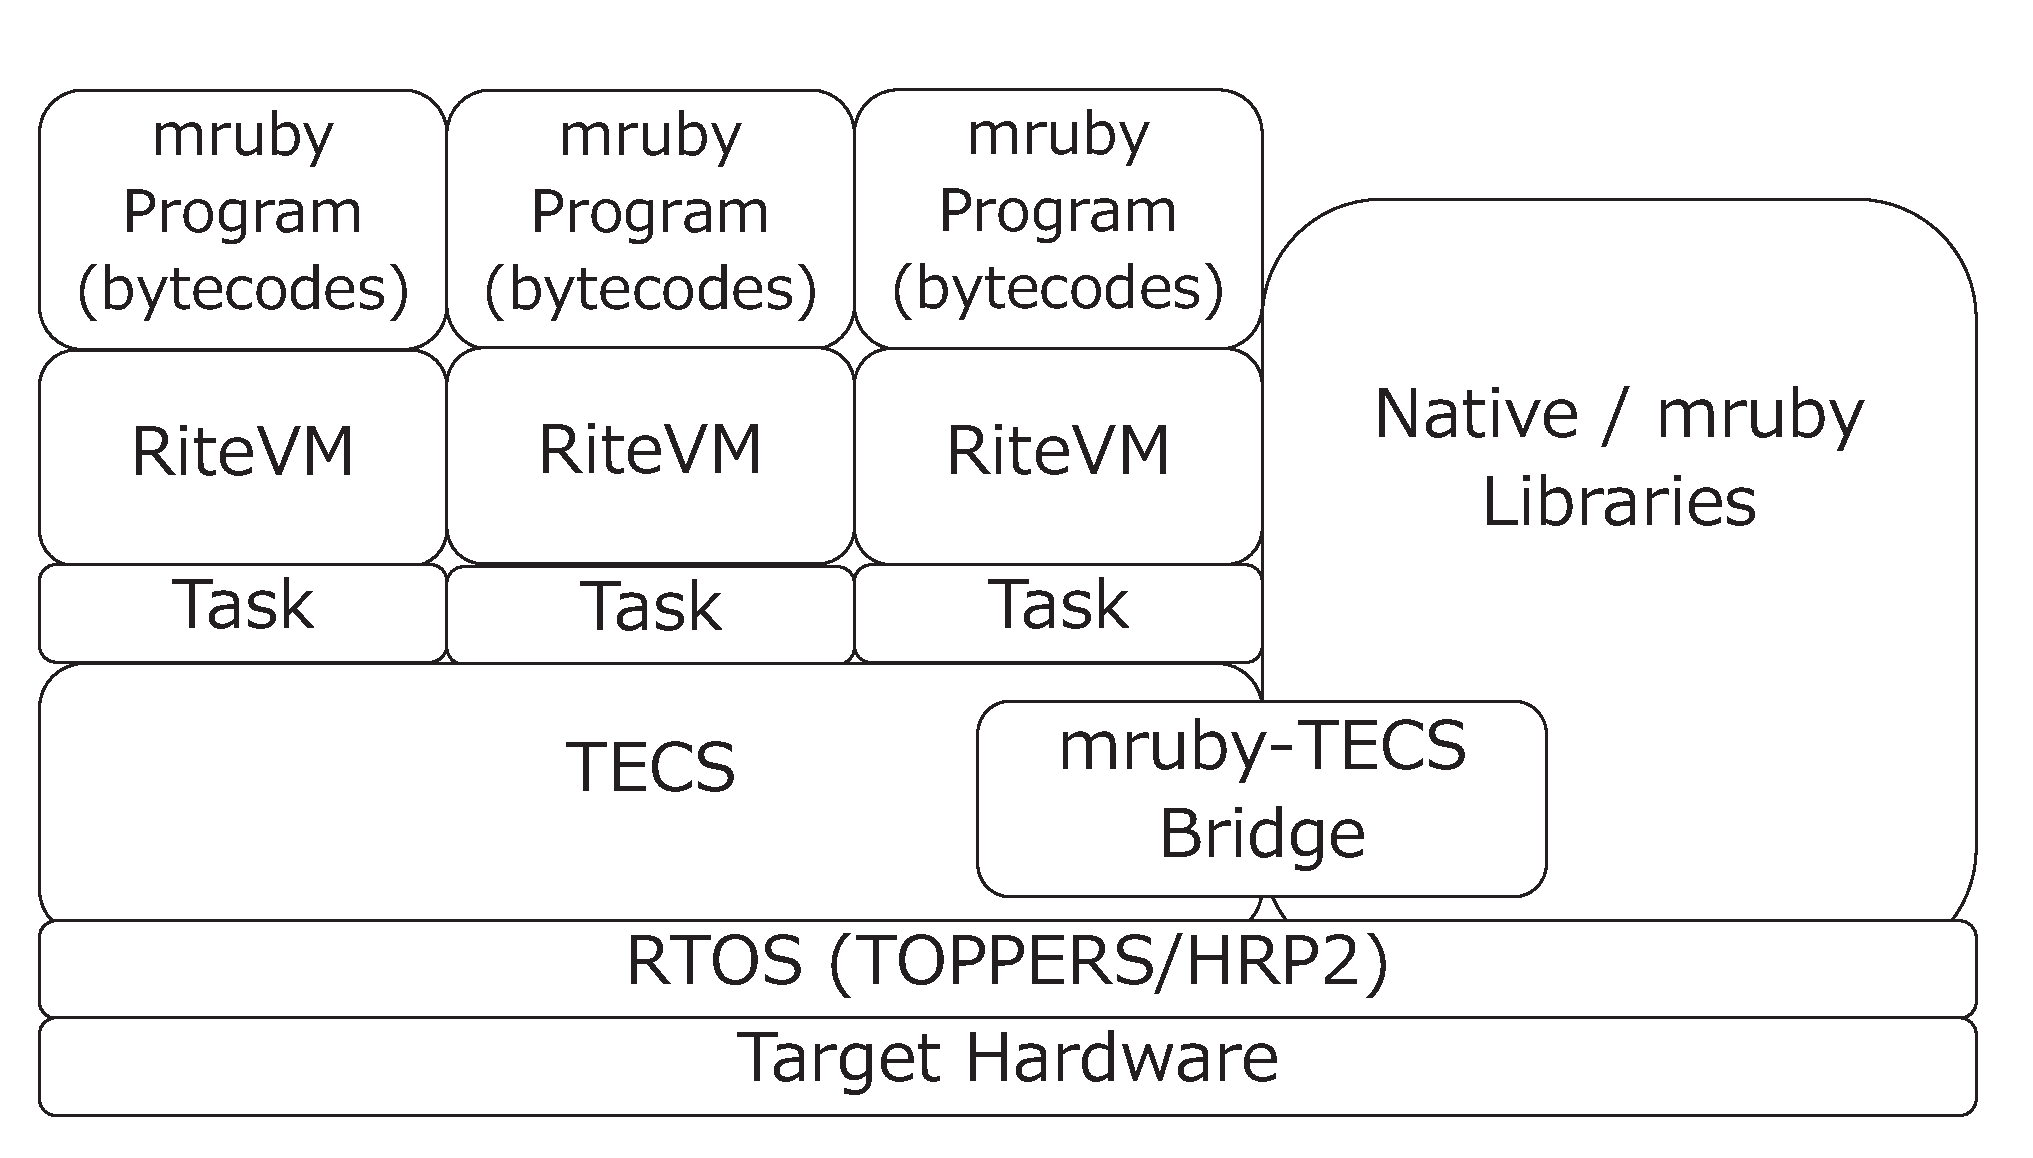
\includegraphics[width=6.5cm,clip]{figure/mrubyontecs.eps}
\caption{System model of existing mruby on TECS}
\label{fig:mrubyontecs}
\end{figure}

\subsubsection{mruby-TECS Bridge}
There is a significant difference between the execution times of mruby and C language codes.
According to  \cite{par:mrubyonTECS}, mruby programs are several hundred times slower than C programs and the execution of an mruby bytecode on a RiteVM is not as efficient as that of C code.
Thus, it is difficult to use mruby exclusively.

Using Ruby on embedded devices improves productivity and maintainability because it is easy to use and read.
However, some C language codes are required to manipulate actuators and sensors and ensure that critical sections of the code run quickly.
% On the other hand, it is necessary to implement parts of applications in C language in order to manipulate actuators and sensors, and also make critical sections of the code run quickly.

Fig.\ref{fig:mruby_TECS_bridge} illustrates an mruby-TECS bridge used to control a motor.
The left side of BridgeMotor belongs to the mruby program.
The right side of BridgeMotor belongs to TECS component.
\begin{figure}[t]
    \centering
    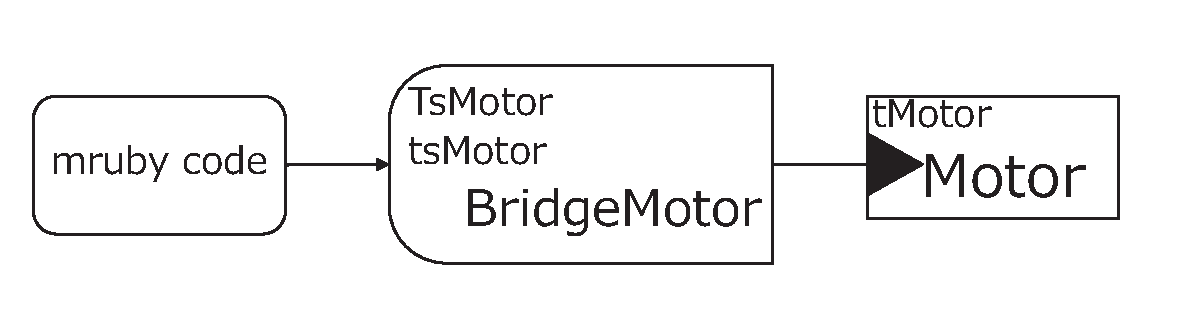
\includegraphics[width=6.5cm,clip]{figure/mruby_TECS_bridge.eps}
\caption{mruby-TECS bridge}
\label{fig:mruby_TECS_bridge}
\end{figure}

The mruby-TECS bridge generates a {\it celltype}, which is called from the mruby code, and an mruby class, which corresponds to a developer-specified TECS component to invoke a C function from the mruby program.

The generated mruby-TECS bridge supports registration of classes and methods for mruby.
Methods in an mruby class are defined by generation codes for an mruby-TECS bridge, such as setPower and stop.
Thus, when a method is called in an mruby program, the mruby-TECS bridge calls the function defined in the TECS component such as a Motor {\it cell}.

\section{Design and Implementation}
\label{sec:Design and Implementation}
Fig.\ref{fig:system_model} shows the detailed system model of the proposed framework.
Each mruby application bytecode transferred from the host to the target device is received by the loader in the RiteVM.
The RiteVM reads the transferred bytecode and executes it with libraries.
The mruby applications run simultaneously due to synchronized processing.
The RiteVM scheduler switches RiteVM tasks because multiple tasks can run concurrently.
The following subsection explains these functionalities.

\begin{figure}[t]
    \centering
    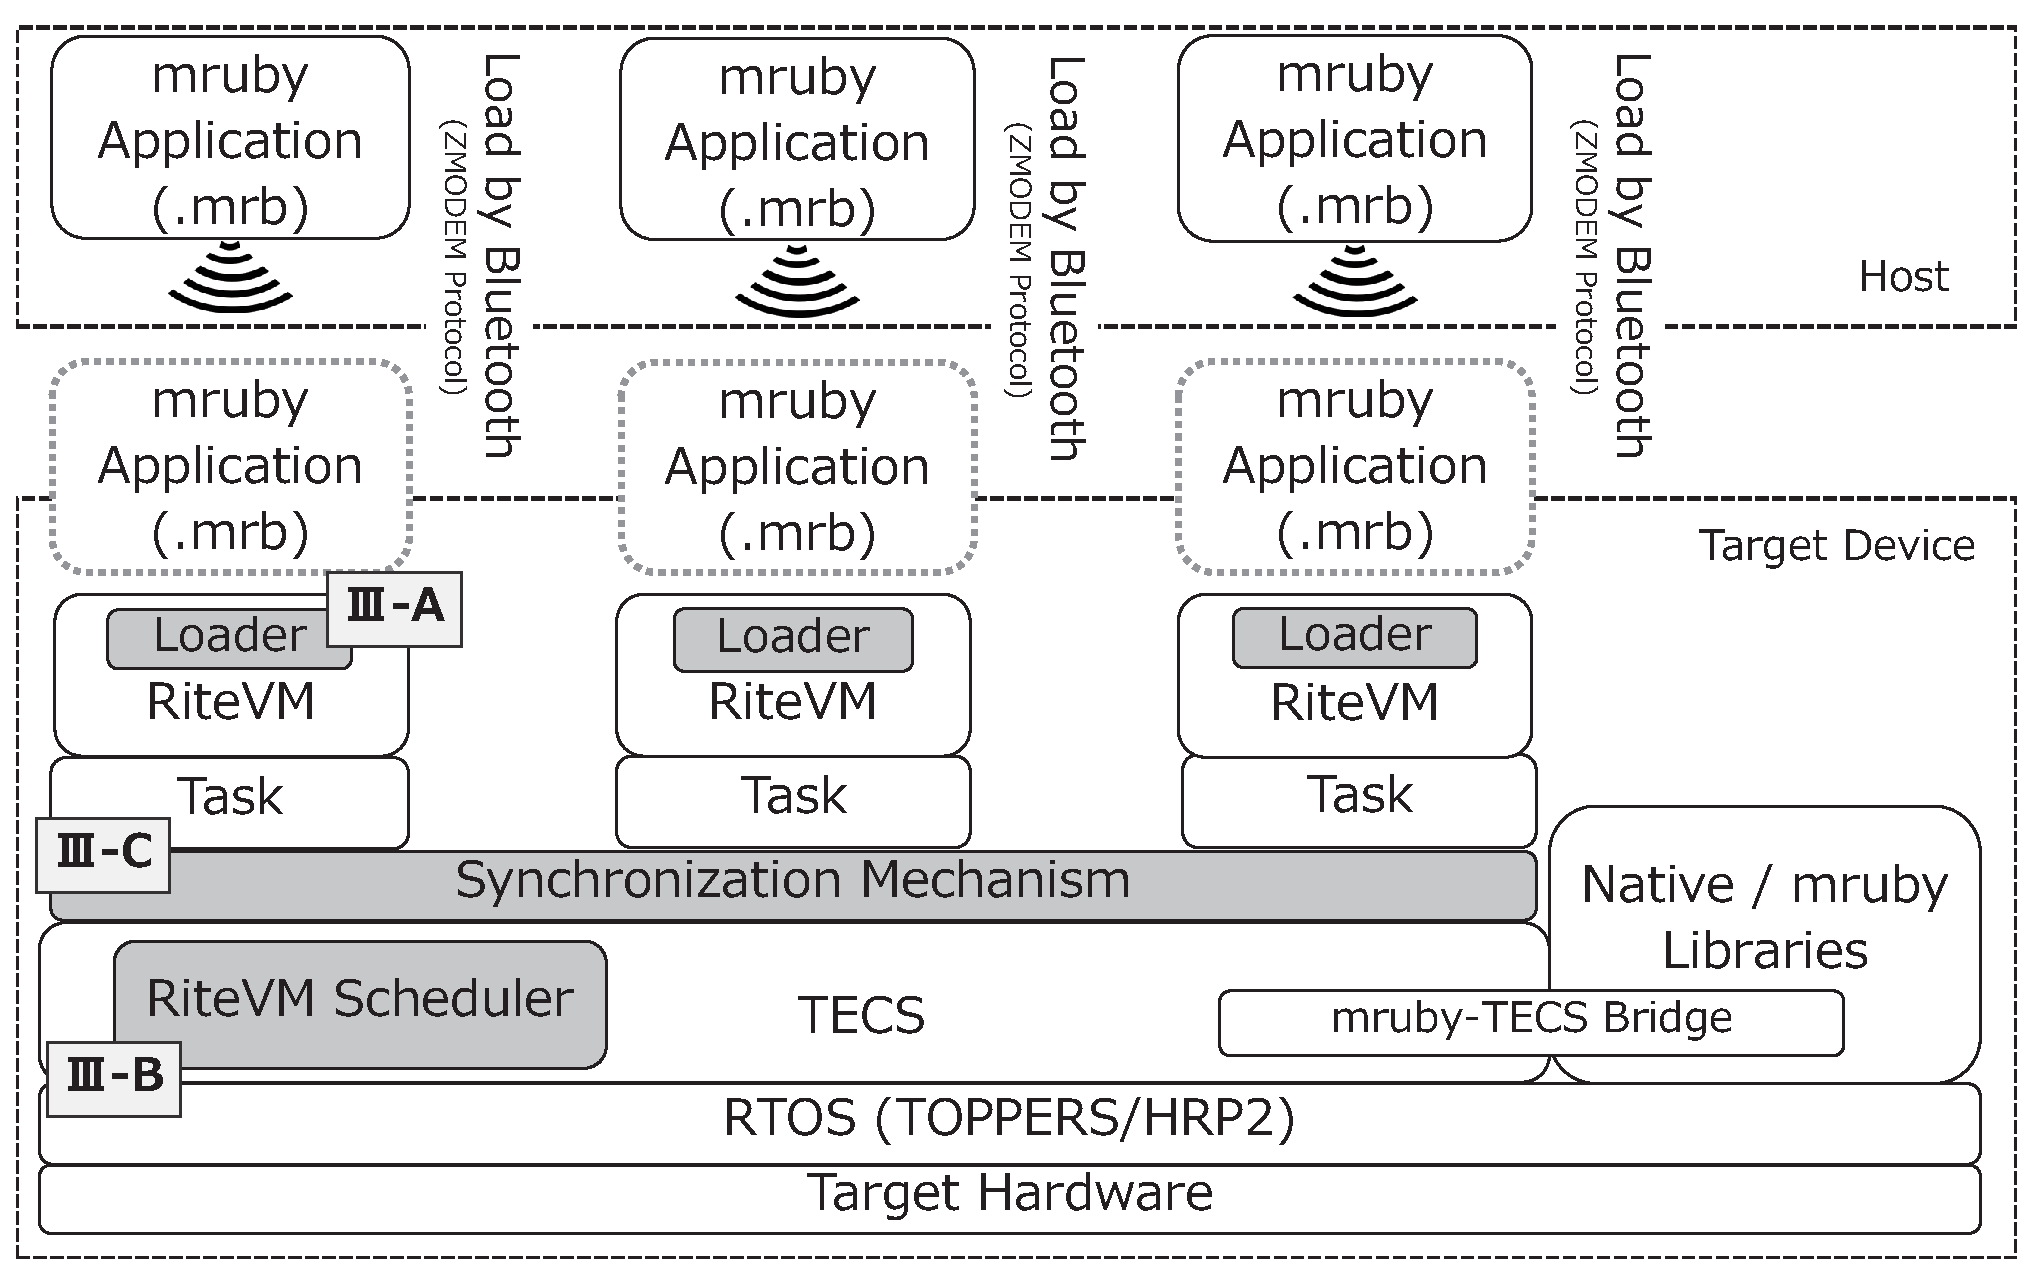
\includegraphics[width=6.5cm,clip]{figure/system_model.eps}
\caption{Detailed system model of the proposed framework}
\label{fig:system_model}
\end{figure}

\subsection{Bluetooth Loader for mruby Bytecode}
\label{sec:Bluetooth loader for mruby bytecode}
This section describes the proposed additional functionality of mruby on TECS, i.e., the Bluetooth loader, for mruby bytecode.\footnote{
The Bluetooth loader is intended to improve development efficiency; therefore, software developers should use it during the development phase.
Note that the complete software should be compiled and linked on the storage/ROM device beforehand.
}
In the current system, the platform including mruby bytecodes is saved on a storage/ROM device.
Developers must rewrite the storage/ROM device every time the programs are modified.
In addition, the RTOS on the target device needs to be restarted.
The repetition hinders development efficiency.
The Bluetooth loader for mruby bytecode decreases developer burden because developers only have to connect the storage/ROM device and start the RTOS once. 

mruby programs consist of an mruby application and mruby libraries.
An mruby application is the main program code, mruby libraries define the functions for the application, such as Ruby classes. 
The mruby bytecodes including both an mruby application and mruby libraries can be transferred and executed on the target device.
However, this is also wasteful in terms of bytecode size and the time required to transfer the bytecodes, because the libraries are not modified frequently.
With the proposed framework, only mruby applications are transferred, and the mruby libraries are preserved on the storage/ROM device beforehand.
As a result, RiteVMs can share mruby libraries.
In addition, a RiteVM can use its own library, which other RiteVMs should not use.

In the proposed framework, a platform that includes RiteVMs and an mruby library is first compiled and copied to the storage/ROM device.
On the host, the mruby application programs (.rb files) are edited and compiled to bytecodes (.mrb files) by an mruby compiler.
The generated bytecodes are transferred from the host to the target device via Bluetooth.
This saves time since Bluetooth pairing can be avoided because the loader can load the bytecode continuously.

\subsubsection{RiteVM Component with Bluetooth Loader for mruby Bytecode}
\begin{figure}[t]
    \centering
    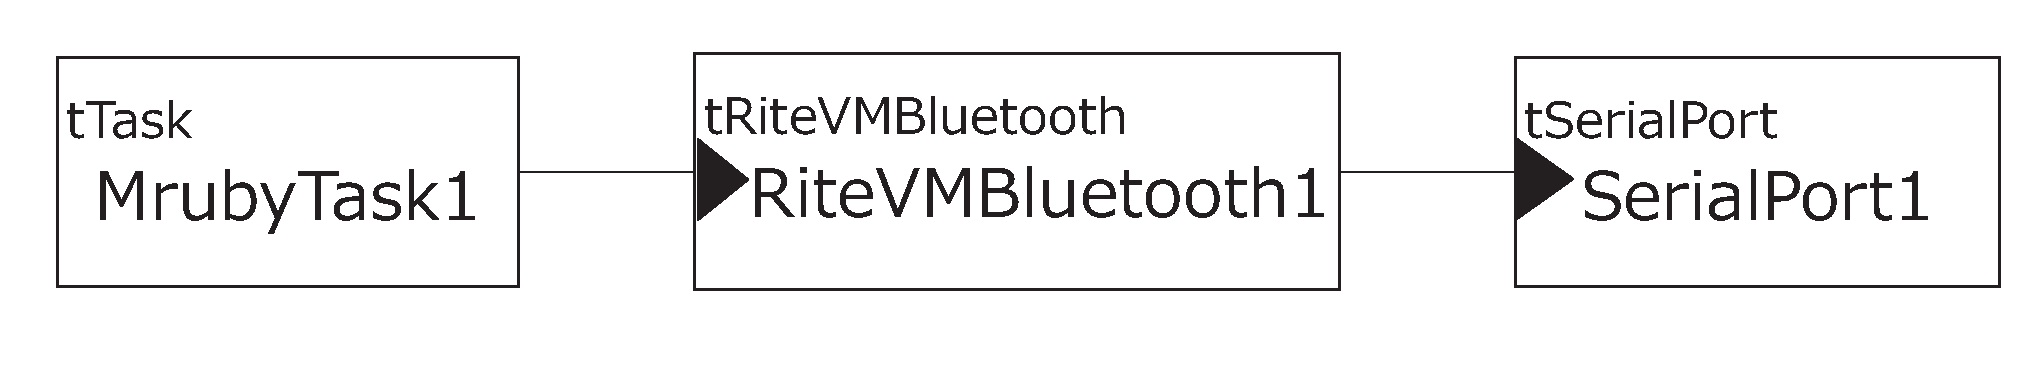
\includegraphics[width=6.5cm,clip]{figure/component_bluetooth.eps}
\caption{Component diagram of Bluetooth loader for mruby bytecode}
\label{fig:component_bluetooth}
\end{figure}
The proposed framework provides a RiteVM with a Bluetooth loader for mruby bytecode as a TECS component.
This component is an extension of the RiteVM component described in \cite{par:mrubyonTECS}.
It receives bytecodes via Bluetooth and manages the RiteVM configuration, such as generating mruby library bytecodes automatically.
This generated bytecode is prepared beforehand on the storage/ROM device and differs from the bytecode transferred with Bluetooth.

Fig.\ref{fig:component_bluetooth} shows a component diagram of MrubyTask1 and RiteVMBluetooth1 {\it cell}s.
The MrubyTask1 {\it cell} is a componentized task of the RTOS (TOPPERS/HRP2 \cite{url:HRP2}, \cite{par:hr-tecs}).
The RiteVMBluetooth1 {\it cell} is the RiteVM component with the Bluetooth loader for mruby bytecode.
Bytecode on the host is transferred and received.
In this framework, ZMODEM \cite{par:zmodem} is used as the binary transfer protocol.

\begin{figure}[t]
    \centering
    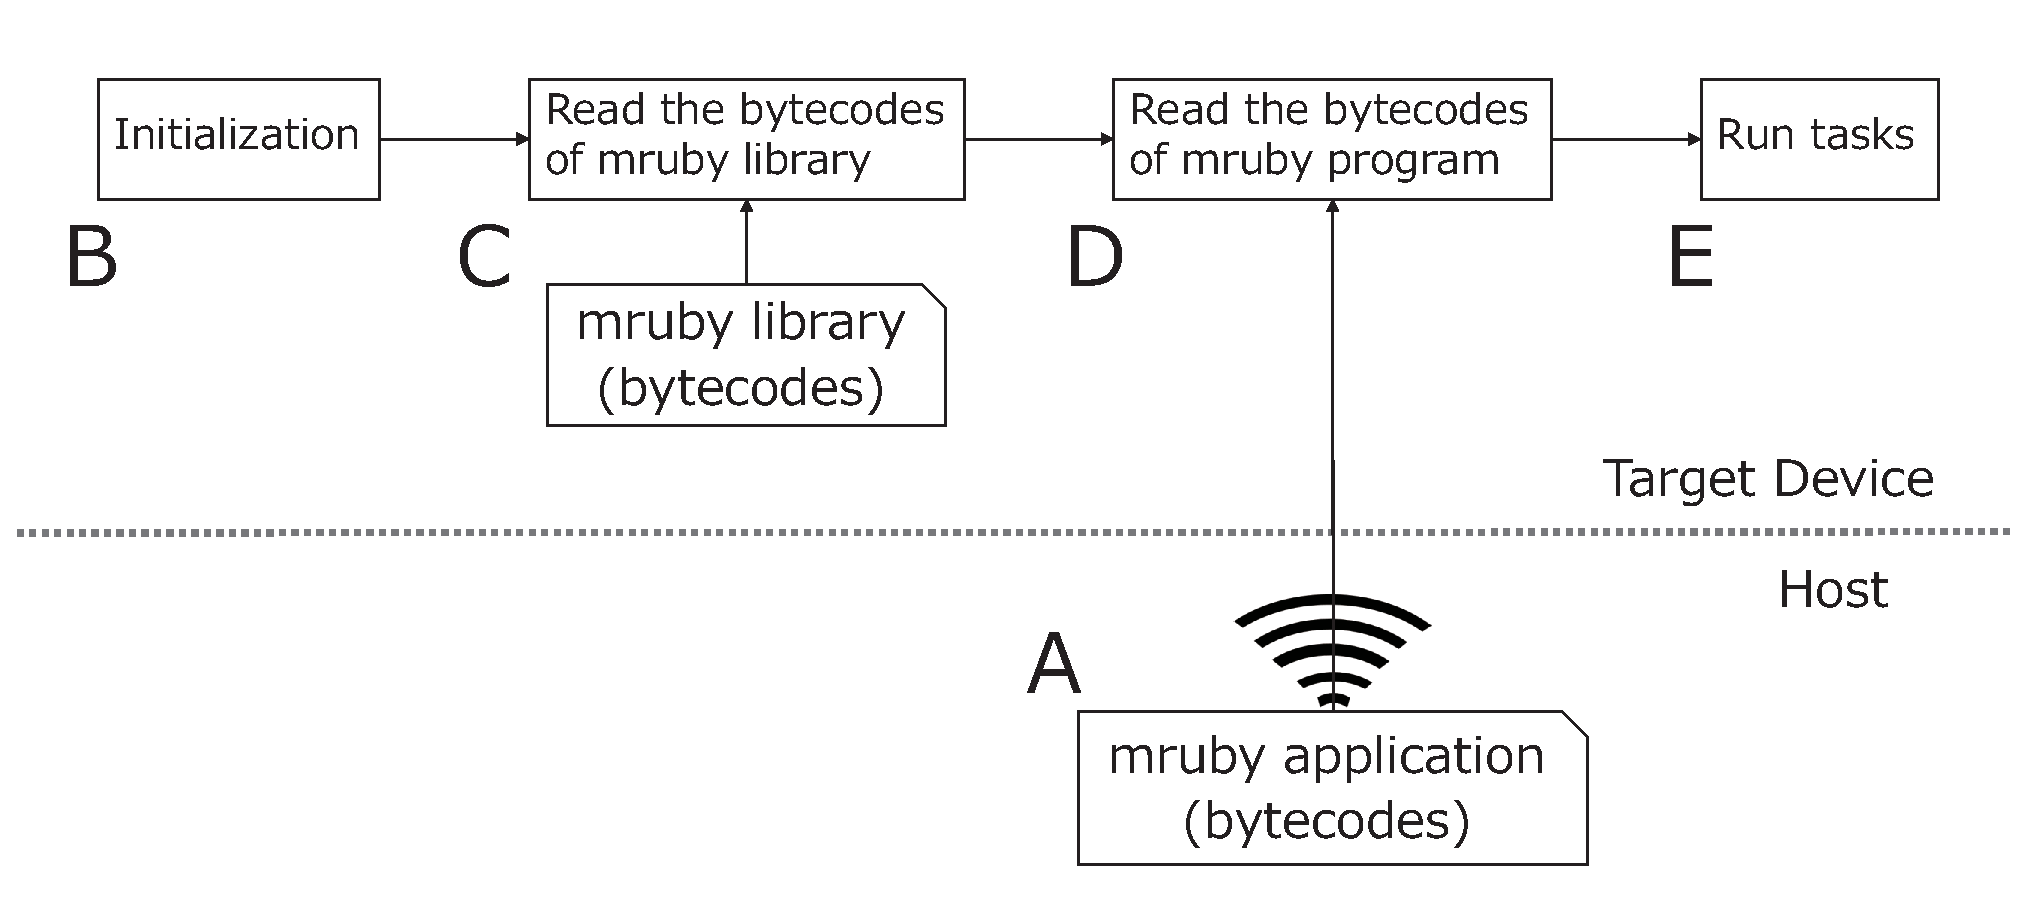
\includegraphics[width=6.5cm,clip]{figure/control_flow.eps}
\caption{Process flow of Bluetooth loader for mruby bytecode}
\label{fig:control_flow}
\end{figure}

\begin{figure}[t]
\centering
\begin{lstlisting}
/* tRiteVMBluetooth.cdl */
celltype tRiteVMBluetooth1 {
    entry sTaskBody eMrubyBody;
    [optional] call sEventflag cEventflag[];
    [optional] call sSemaphore cSemaphore;
    attr {
      [omit]char_t *mrubyLib;
      char_t *irepLib = 
                C_EXP("&$cell_global$_irep");
      uint32_t irepAppSize = 
                C_EXP( BUFFER_SIZE );
      FLGPTN setptn;
    };
    var {
        mrb_state *mrb;
        mrbc_context *context;
        [size_is(irepAppSize)] uint8_t *irepApp;
    };
};
\end{lstlisting}
\caption{Celltype description for RiteVM with Bluetooth loader for mruby bytecode}
\label{celltype_mrubybluetooth}
\end{figure}

\begin{figure}[t]
\centering
\begin{lstlisting}
/* tRiteVMBluetooth.c */
void eMrubyBody_main( CELLIDX idx )
{
 /* Omit: start of exclusive process by semaphore */
 /* Receive the bytecode via Bluetooth */
 bluetooth_loader( VAR_irepApp );
 /* Omit: end of exclusive process by semaphore */
 /* New interpreter instance */
 VAR_mrb = mrb_open();
 /* Omit: error check for mrb_state */
 /* New mruby context */
 VAR_context = mrbc_context_new(VAR_mrb);
 /* Omit: initialize mruby-TECS bridge */
 /* Omit: synchronization of
        initializing mruby application */
 /* Load mruby library bytecode */
 mrb_load_irep_cxt( VAR_mrb,
                    ATTR_irepLib,
                    VAR_context );
 /* Load mruby application bytecode and run */
 mrb_load_irep_cxt( VAR_mrb,
                    VAR_irepApp,
                    VAR_context );
 if ( mrb->exc ) {
   /* Failure to execute */
   mrb_p( VAR_mrb, 
          mrb_obj_value( VAR_mrb->exc ) );
   exit( 0 );
 }
 /* Omit: synchronization of
           terminating mruby application */
 /* Free mruby context */
 mrbc_context_free( VAR_mrb, VAR_context );
 /* Free interpreter instance */
 mrb_close( VAR_mrb );
}

\end{lstlisting}
\caption{Main code for RiteVM with Bluetooth loader for mruby bytecode}
\label{maincode_mrubybluetooth}
\end{figure}

Fig.\ref{fig:control_flow} shows the process flow for executing an mruby program on the RiteVM component with the Bluetooth loader for mruby bytecode, such as RiteVMBluetooth1.
The main tRiteVMBluetooth code is shown in Fig.\ref{maincode_mrubybluetooth}.

First, the Bluetooth loader receives the mruby application bytecode from the host (Fig.\ref{fig:control_flow}(A); lines 5-6 in Fig.\ref{maincode_mrubybluetooth}).
The bytecode is stored in a component variable, such as {\it VAR\_irepApp}, as shown in Fig.\ref{celltype_mrubybluetooth}.
This process is exclusively carried out by the semaphore to prevent the other loading from interrupting.

Second, {\it mrb\_state} and {\it mrbc\_context} pointers, and mruby-TECS bridges are initialized (Fig.\ref{fig:control_flow}(B); lines 8-13 in Fig.\ref{maincode_mrubybluetooth}).
{\it VAR\_mrb} and {\it VAR\_context} show the variables of the {\it cell}.
{\it mrb\_state} is a set of states and global variables used in mruby.
The synchronization of multiple tasks is performed in this processing phase.
The RiteVM that finishes execution at this point waits for the another RiteVM to finish loading and initialization.

Third, the RiteVM reads the bytecode of mruby libraries (Fig.\ref{fig:control_flow}(C); lines 16-19 in Fig.\ref{maincode_mrubybluetooth}).
The mruby libraries are a set of Ruby classes, such as the motor and sensor classes.
For example, the motor class defines methods to rotate and stop a motor.
The tRiteVMBluetooth {\it cell} has the attributes shown in Fig.\ref{celltype_mrubybluetooth}.
{\it ATTR} indicates an attribute which is a fixed value that cannot be rewritten, unlike {\it VAR}.
The {\it mrubyLib} indicates the program files of the mruby libraries, and is an attribute because mruby libraries are not modified in the proposed development process.
Here, {\it [omit]} is only used for the TECS generator; thus, the attribute {\it mrubyLib} does not consume memory.
{\it irepLib} is the pointer of the array in which the bytecode of mruby libraries is stored.
To summarize, the bytecode of mruby libraries is stored as an attribute of the component during the first compilation.

Fourth, the RiteVM reads the bytecode of the mruby application transferred via Bluetooth (Fig.\ref{fig:control_flow}(D); lines 20-23 in Fig.\ref{maincode_mrubybluetooth}).
The mruby application bytecode is stored in an array of {\it irepApp}, which differs from the array that holds the mruby library bytecode.
Note that two bytecodes are read separately in the RiteVM.

Finally, the mruby task runs (Fig.\ref{fig:control_flow}(E); lines 20-23 in Fig.\ref{maincode_mrubybluetooth}).
When an mruby application is modified, only the bytecode of the modified application should be transferred; the mruby libraries do not need to be touched because they typically do not change.

The process shown in Fig.\ref{maincode_mrubybluetooth} (lines 24-29) is carried out when an exception occurs.
When all mruby applications are completed, mrb\_state and mrbc\_context are freed (lines of 32-35 in Fig.\ref{maincode_mrubybluetooth}).
The proposed framework supports continuous loading; thus, this process loops.
After the variables are freed, the RiteVM waits for the next mruby application bytecode.

\subsection{RiteVM Scheduler}
\label{sec:RiteVM Scheduler}
This section describes the implementation of the RiteVM scheduler in the proposed framework.
mruby on TECS supports multitasking; however, multitask processing in mruby on TECS requires the developers to have knowledge about the RTOS (TOPPERS/HRP2).

One approach for multitasking is a co-routine, which is a cooperative thread scheduled by developers with functions such as {\it resume} and {\it yield} (the Ruby co-routine is defined in the Fiber class \cite{url:co-routine}).
A co-routine is non-preemptive multitasking, which does not receive OS support because developers must switch tasks manually.
A co-routine cannot take advantage of multicore processing.

As another method, {\it delay()}, which is a service call of $\mu$ITRON, can be used for multitasking.
This service call delays the execution of its own task for the time of the argument.
{\it delay()} is needed when scheduling fixed-priority tasks.
However, the programming applied to {\it delay()} is difficult to use with fair scheduling.

For multitask processing, the proposed framework provides the RiteVM scheduler, which is a fair scheduler that runs multiple tasks equally.
Note that the RiteVM scheduler is utilized only when application tasks have equal priority.
mruby applications can run concurrently without calling an OS function.
The application programs can also utilize existing programs because their structures do not change.

The RiteVM scheduler is a fair scheduler that is implemented as a TECS component in the proposed framework.
Therefore, when developers create software with priority-based scheduling, the RiteVM scheduler can be removed easily.

\begin{figure}[t]
    \centering
    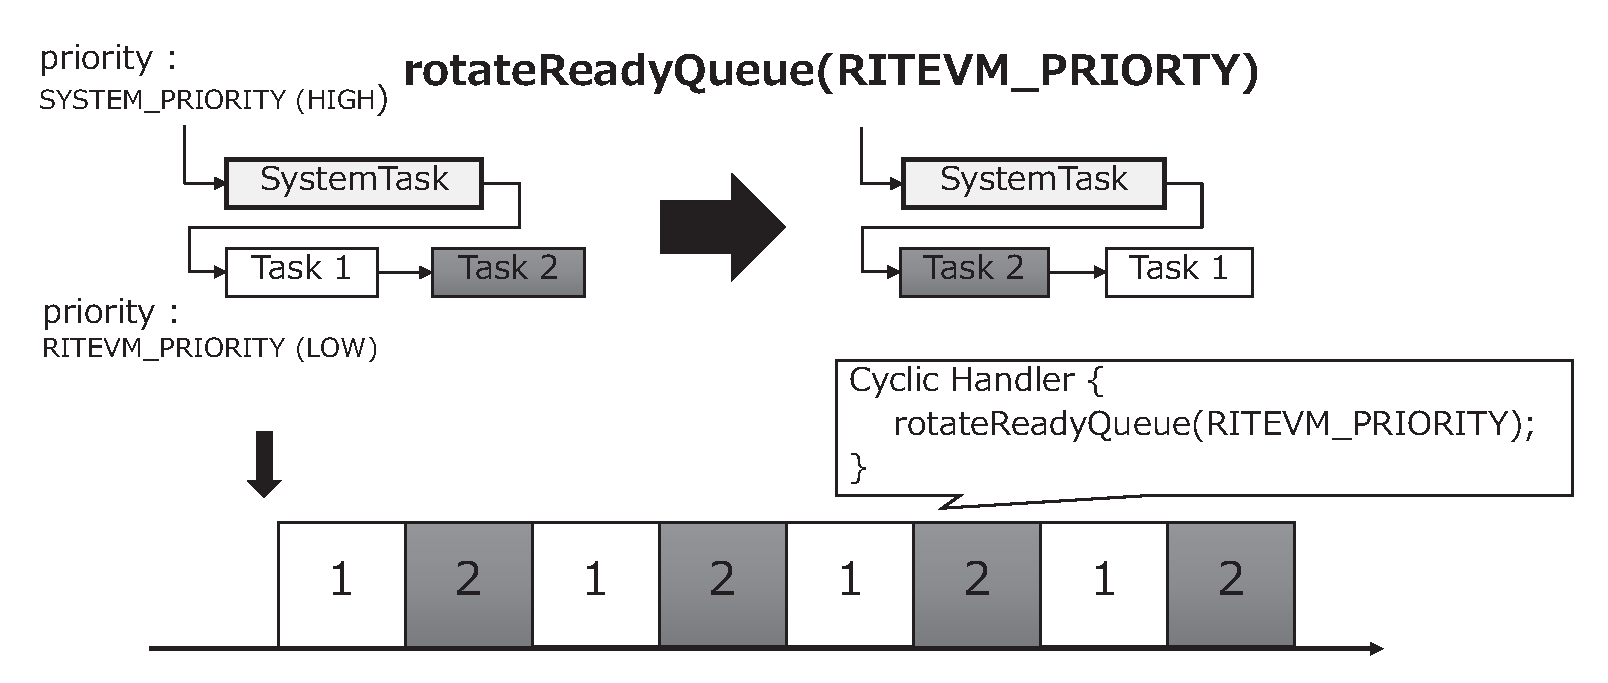
\includegraphics[width=6.5cm,clip]{figure/rotateReadyQueue.eps}
\caption{RiteVM scheduler design}
\label{fig:rotateReadyQueue}
\end{figure} 
\begin{figure}[t]
    \centering
    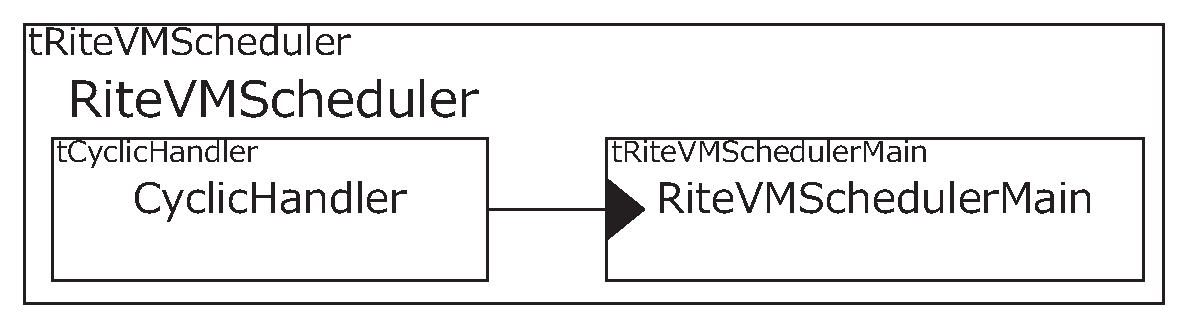
\includegraphics[width=6.5cm,clip]{figure/cyclic_handler.eps}
\caption{Component diagram of RiteVM scheduler}
\label{fig:cyclic_handler}
\end{figure}


\subsubsection{RiteVM Scheduler Design}
A RiteVM scheduler is a periodic handler, and {\it rotateReadyQueue}, which is a service call of $\mu$ITRON to switch tasks with equal priority, is implemented as the main process of the handler.
In other words, the RiteVM scheduler calls {\it rotateReadyQueue} cyclically.
The design of the RiteVM scheduler is shown in Fig.\ref{fig:rotateReadyQueue}. 
{\it rotateReadyQueue} is described as follows.

Here, assumed that two tasks with equal priority are in an infinite loop.
In the current system, when one task is executed first, the other task would not be executed because the first task runs in the loop.

When {\it rotateReadyQueue} is called, tasks with equal priority are switched as shown in Fig.\ref{fig:rotateReadyQueue}.
Note that the argument of {\it rotateReadyQueue} is the priority.

In addition, {\it rotateReadyQueue} can be performed if the number of tasks is more than two.
For example, three tasks are in the order task1, task2, and task3.
In this case, the order is rotated to task2, task3, and task1 when {\it rotateReadyQueue} is called.

\begin{figure}[t]
    \centering
    \begin{lstlisting}
/* tRiteVMScheduler.cdl */
celltype tCyclicHandler {
  [inline] entry sCyclic eCyclic;
  call siHandlerBody  ciBody;
  attr {
      [omit] ATR    attribute   =
                      C_EXP("TA_NULL");
      [omit] RELTIM cyclicTime;
      [omit] RELTIM cyclicPhase;
  };
};
celltype tRiteVMSchedulerMain {
  require tKernel.eiKernel;
  entry   siHandlerBody eiBody;
  attr {
      PRI priority;
  };
};

composite tRiteVMScheduler {
  attr {
      ATR    attribute      = C_EXP("TA_NULL");
      RELTIM cyclicTime  = 1;
      RELTIM cyclicPhase = 1;
      PRI    priority;
  };
  cell tRiteVMSchedulerMain RiteVMSchedulerMain {
      priority = composite.priority;
  };
  cell tCyclicHandler CyclicHandler {
      ciBody      = RiteVMSchedulerMain.eiBody;
      attribute   = composite.attribute;
      cyclicTime  = composite.cyclicTime;
      cyclicPhase = composite.cyclicPhase;
  };
};
\end{lstlisting}
\caption{Celltype description of RiteVM scheduler}
\label{celltype_cyclic_handler}
\end{figure}
\begin{figure}[t]
    \centering
    \begin{lstlisting}
cell tRiteVMScheduler RiteVMScheduler {
    attribute   = C_EXP("TA_STA");
    cyclicTime  = 1;
    cyclicPhase = 1;
    priority    =
        C_EXP("RITEVM_PRIORITY");
};
\end{lstlisting}
\caption{Build description of RiteVM scheduler}
\label{build_cyclic_handler}
\end{figure}

\subsubsection{Component of RiteVM Scheduler}

Fig.\ref{fig:cyclic_handler} shows a component diagram of the RiteVM scheduler.
The RiteVM scheduler is a {\it composite cell} which consists of CyclicHandler and RiteVMSchedulerMain.
The CyclicHandler {\it cell} configures the periodic handler based on $\mu$ITRON.
Cyclic handlers based on $\mu$ITRON are described in the literature \cite{par:microITRON}.
The CyclicHandler {\it cell} has the attributes of the {\it cell}.
The RiteVMSchedulerMain {\it cell} processes the body of a periodic handler.
Note that {\it rotateReadyQueue} is implemented as the body.
Fig.\ref{celltype_cyclic_handler} shows tRiteVMScheduler {\it celltype}, which is a {\it composite cell} consisting of two {\it cell}s.
The {\it call} port of RiteVMSchedulerMain is connected to the {\it entry} port of the Kernel {\it cell} ({\it tKernel.eiKernel}) to call kernel functions.
The attribute is used as the {\it rotateReadyQueue} arguments.

Fig.\ref{build_cyclic_handler} shows the build description of the RiteVM scheduler.
The RiteVMScheduler {\it cell} has attributes to configure the scheduler such as attribute, cyclicTime, cyclicPhase, and priority.
In this case, the RiteVM scheduler is executed when it is generated, because the attribute is {\it TA\_STA}, which indicates that the periodic handler is in an operational state after creation.
Note that the scheduler executes every 1 msec.
RITEVM\_PRIORITY defines the priority of mruby tasks.
In the function of RiteVMSchedulerMain, {\it rotateReadyQueue} is implemented and the priority is passed as the argument.


\begin{figure}[t]
    \centering
    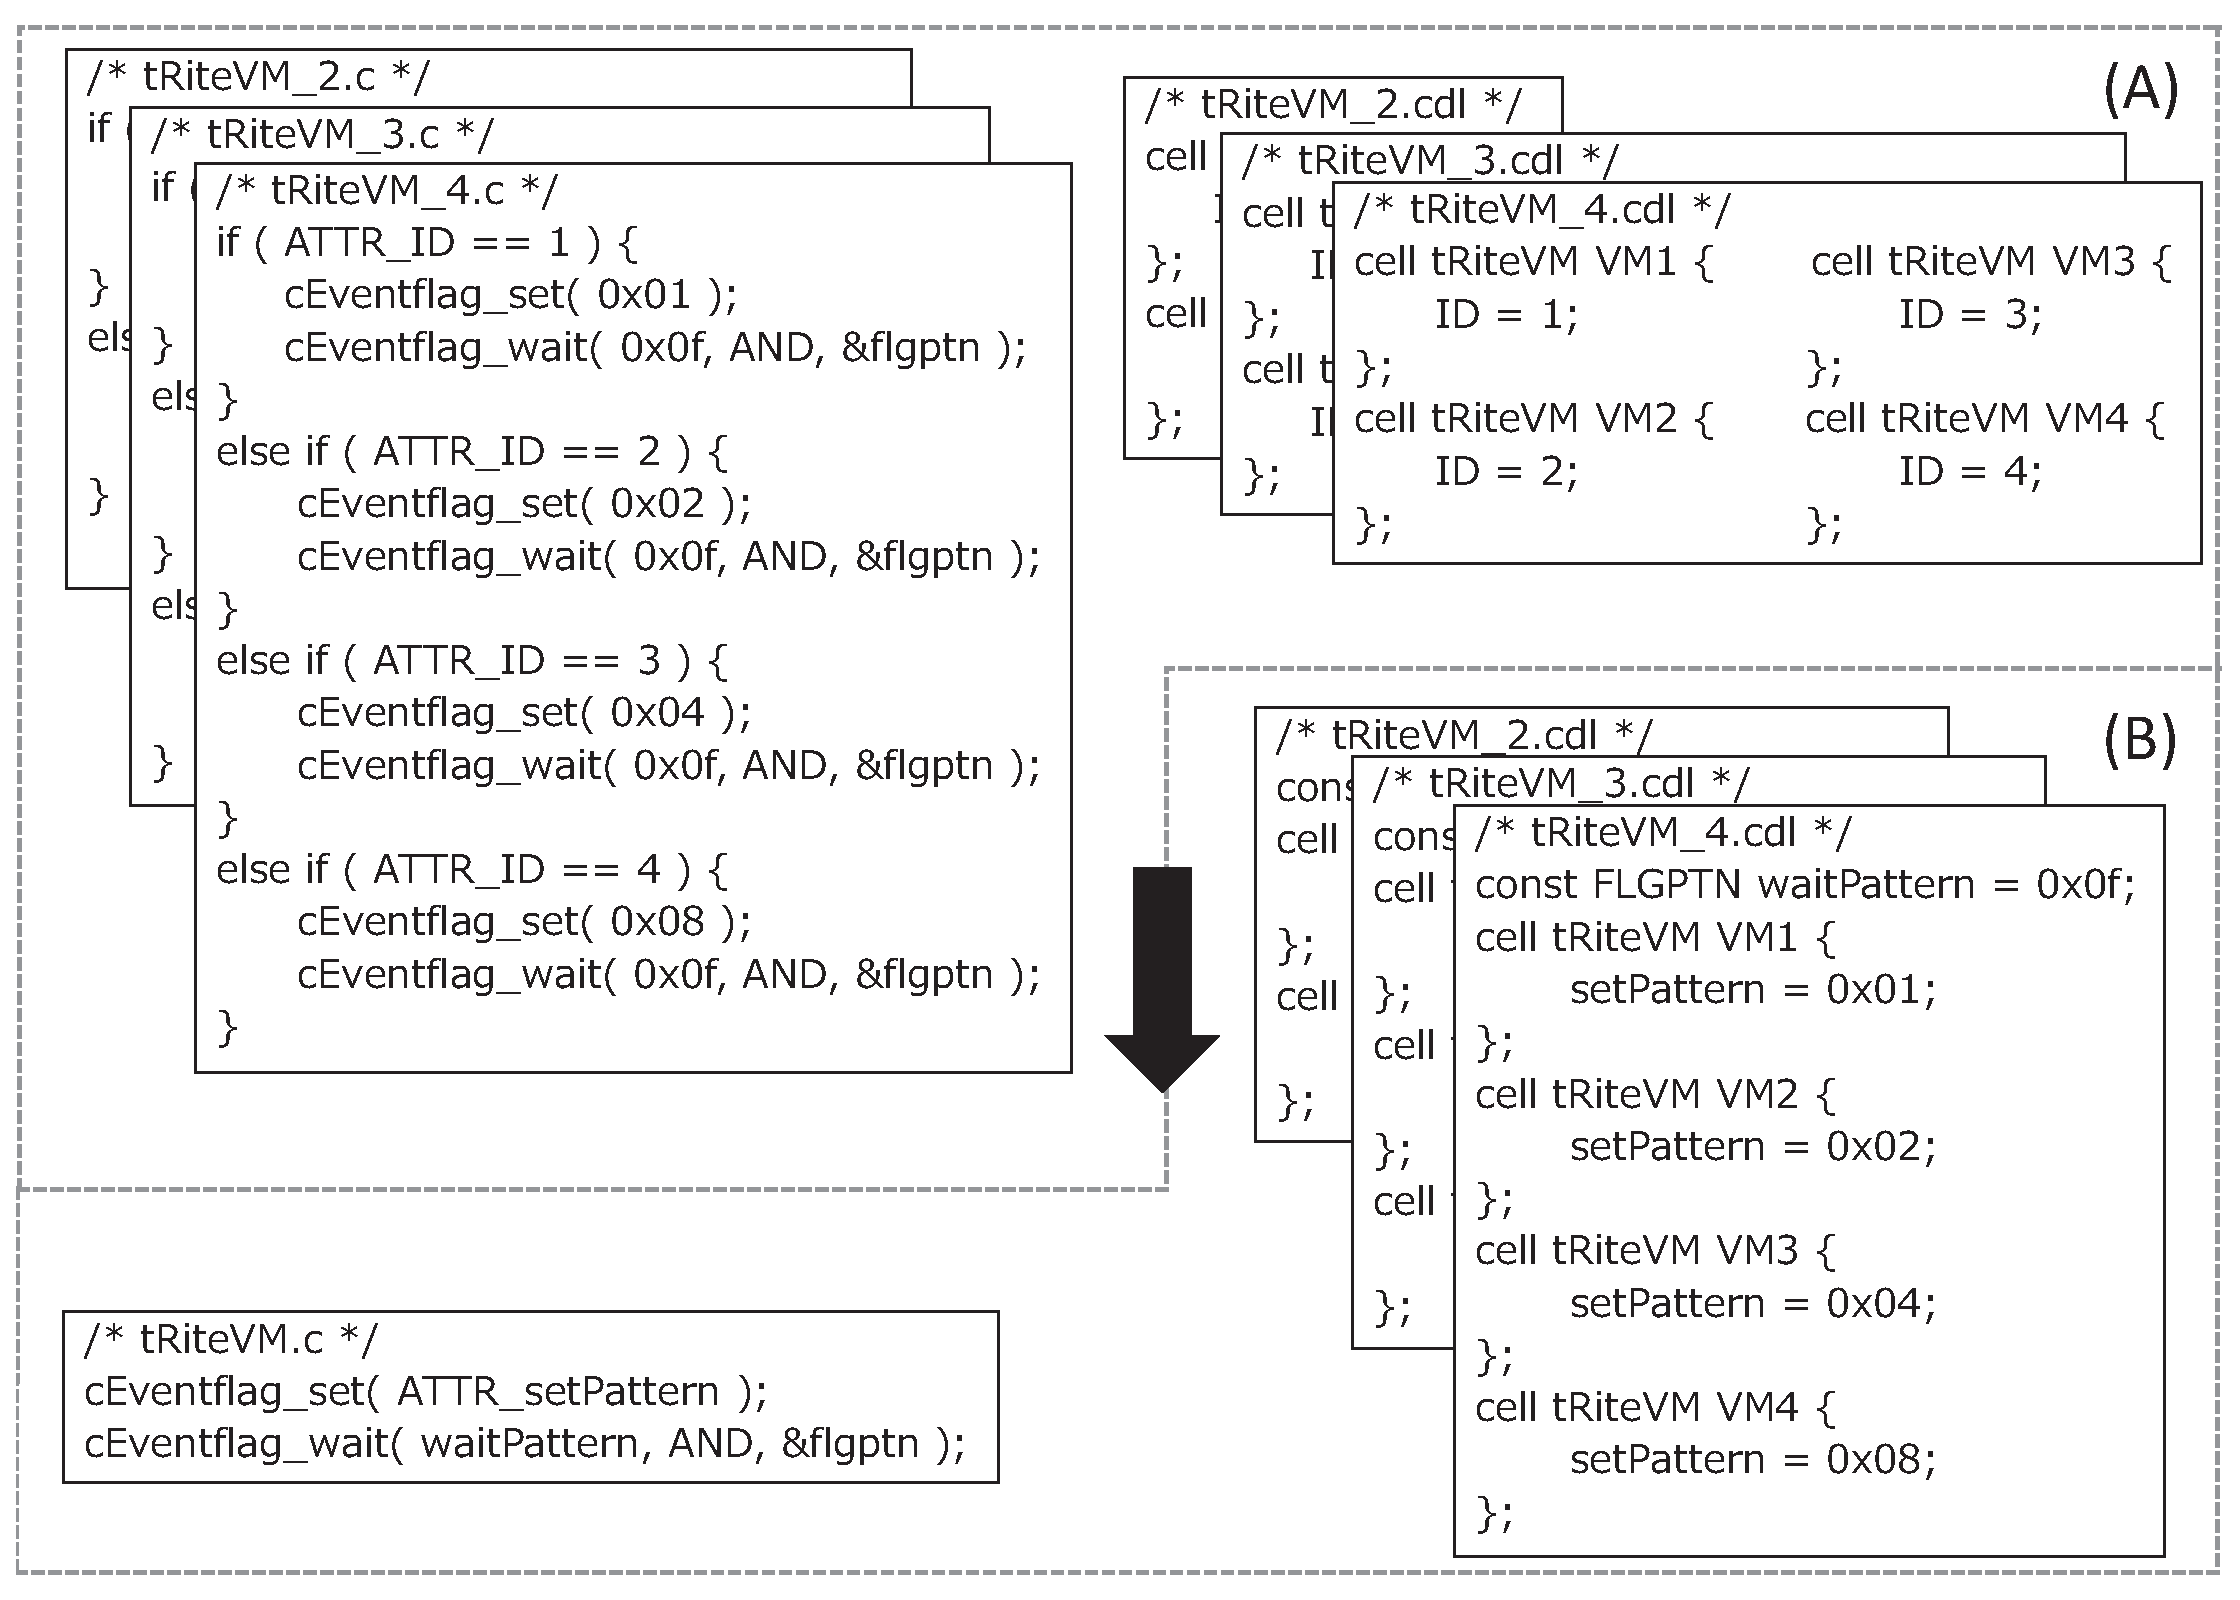
\includegraphics[width=6.5cm,clip]{figure/Eventflag.eps}
\caption{Design of Eventflag using TECS (only differences are shown)}
\label{fig:Eventflag}
\end{figure}

\subsection{Synchronization of Multiple RiteVM Tasks}
In the proposed framework, RiteVMs read mruby bytecodes and then execute applications.
Eventflag is applied to synchronize the initiation of multiple mruby applications.
Each task sets a flag pattern, such as 0x01 (01) and 0x02 (10), and then waits for the flag pattern 0x03 (11) with AND.
This process can also be applied to more tasks.
For example, for four RiteVM tasks, each task sets a flag pattern, such as 0x01 (0001), 0x02 (0010), 0x04 (0100), and 0x08 (1000), and then waits 0x0f (1111) with AND, as shown in Fig.\ref{fig:Eventflag}(A).

In addition, the termination of mruby applications is synchronized to accept continuous loading.
This termination synchronization prevents a RiteVM whose application finishes immediately from waiting for the next loading.
Thus, all mruby applications finish at the same time, and all RiteVMs wait to receive the next mruby application bytecodes. 

 
\subsection{Utilization of Component-Based Development}
% This section describes the design applying component-based development.
In the proposed framework, RiteVMs, the RiteVM scheduler, and Eventflags are implemented as components.
Therefore, developers can add, remove, or reuse these components easily.
For example, if the RiteVM scheduler is not necessary for the software, developers should comment out only the CDL file, e.g., {\it //import("tRiteVMScheduler.cdl");}.
CBD eliminates the need for developers to rewrite kernel configuration files.

In addition, the code size can be reduced by using CBD. 
In the proposed framework, this advantage is applied in the Eventflag component.
The set pattern and wait pattern are defined as attributes of the component as shown in Fig.\ref{fig:Eventflag} (B).
This design, e.g., {\it cEventflag\_set(ATTR\_setPattern)}, enables the program without ``if'' statements and reuses an identical C file.
Developers do not need to modify the C file because the CDL files are prepared according to the number of RiteVMs.
In addition, the Eventflag components are built with {\it [optional]} in TECS.
Here, {\it [optional]} means that the code is run only when the call port is connected.
Thus, the C file does not need to be rewritten even if the Eventflag is not used. 



\section{Experimental Evaluation}
\label{sec:Evaluation}
This section discusses experimental results.
To analyze the advantages of the proposed framework, we evaluated the following.
\begin{itemize}
    \item Execution time of the platform
    \item Size and time of transferred mruby bytecodes by the Bluetooth loader
    \item Execution time with singletasking, co-routine, and proposed multitasking
    \item Overhead for periodic time
    \item Synchronization of multiple RiteVM tasks
    \item Code size with CBD 
\end{itemize}

These evaluations were performed to demonstrate that a Bluetooth loader can improve the efficiency of software development, that the proposed multitask processing executes effectively compared to singletasking or co-routine, and that the initiation of mruby applications are synchronized.
In addition, we focused on benefits of CBD.
We implemented the proposed system on a LEGO MINDSTORMS EV3 \cite{par:EV3} (300MHz ARM9-based Sitara AM1808 system-on-a-chip) compiled with gcc 4.9.3 -O2 and mruby version 1.2.0.


\subsection{Improving Software Development Efficiency by Bluetooth Loader}

\begin{table}[t]
    \centering
\caption{Development procedure of existing and proposed frameworks}
    \scriptsize
    {\tabcolsep=0.1cm
    \begin{tabular}{c||c}
                            & Development procedure \\ \hline
        Exisiting framework &    (1) + (2) + (3)    \\ %\hline
        Proposed framework  &          (4)          \\ \hline
        \multicolumn{2}{l}{ (1): Rewrite the storage device} \\
        \multicolumn{2}{l}{ (2): Insert the storage device into the target} \\
        \multicolumn{2}{l}{ (3): Restart the RTOS on the target (about 4 sec)} \\
        \multicolumn{2}{l}{ (4): Transfer an mruby bytecode from host to target} \\
    \end{tabular}
    }
    \label{tab:procedure}
\end{table}

\begin{table}[t]
    \centering
\caption{Size and load process time of an mruby application with/without libraries}
    \scriptsize
    {\tabcolsep=0.1cm
    \begin{tabular}{c||c|c|c}
                        & App\&Lib     & App        &   App\&Lib/App  \\ \hline
        Bytecode Size   & 14,044 bytes & 199 bytes  &   $\times$70.6          \\ %\hline
        Loading Time    & 305.081 msec & 7.774 msec &   $\times$39.2          \\
        Compile Time    & 8.7 msec     & 0.3 msec   &   $\times$29.0          \\
    \end{tabular}
    }
    \label{tab:size_and_time}
\end{table}

The Bluetooth loader for mruby bytecode can reduce the development time.
With the proposed framework, developers do not need to rewrite a storage/ROM device because only the bytecode should be transferred.
In the proposed framework, the development procedure is shortened as shown Table \ref{tab:procedure}
For example, with the existing system, when mruby programs are modified, developers must remove an SD card from the target device, connect the host PC, compile/link the platform, and reinsert the SD card in the target device in an experimental environment such as LEGO MINDSTORMS EV3.
In addition, the proposed framework eliminates the need to restart the target RTOS.
Note that the time of restarting the RTOS, including initializing device drivers, is 4 sec in case of the EV3 platform \cite{par:EV3}

%\subsubsection{Size and time for transferred mruby bytecodes}
In the proposed framework, to further improve software development efficiency, developers transfer only the mruby application bytecode; mruby libraries are incorporated in the platform.
The size, load process time, and compilation time for an mruby application with and without mruby library are shown in Table \ref{tab:size_and_time}.
The overhead of load processing to load a zero byte bytecode is 50.933 msec.
Similarly, compilation overhead to compile a zero byte program is 46.9 msec.
The mruby application bytecode is smaller and faster than including the mruby libraries for all terms.
The difference increases as the number of RiteVMs increases because 50 msec of overhead is incurred per RiteVM. 
These advantages improve the efficiency of software development.


\subsection{RiteVM Scheduler}

\begin{figure}[t]
    \centering
    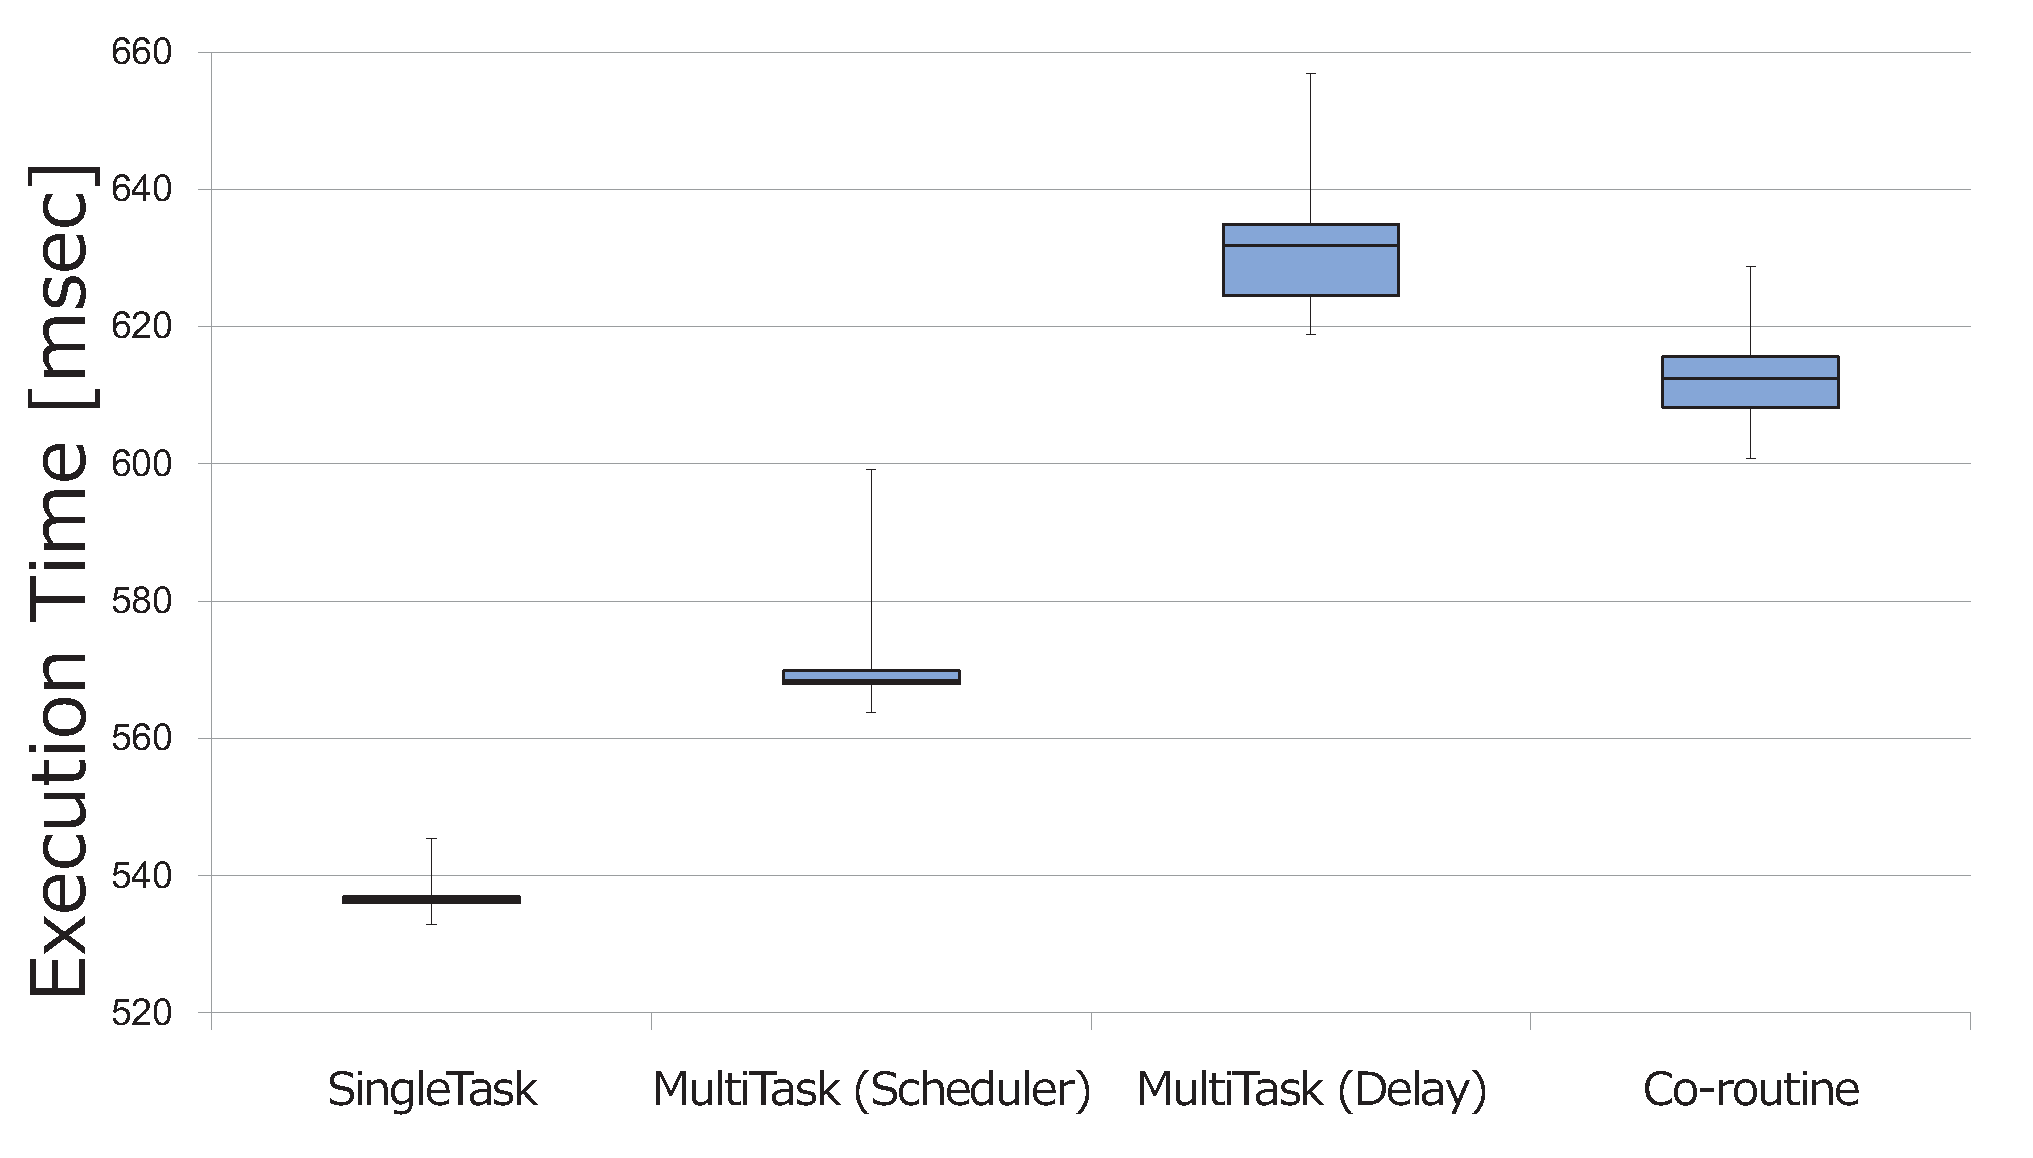
\includegraphics[width=6.5cm,clip]{figure/comparison_s_c_m.eps}
\caption{Comparison of application execution time with singletask, co-routine, and multitask}
\label{fig:comparison_s_c_m}
\end{figure}

% A comparison of the application execution time with singletasking, co-routine, and multitasking is shown in Fig.\ref{fig:comparison_s_c_m}.
% A program with 100,000 loops was used as an mruby application for the evaluation of execution time.
% Here, the singletask program looped 100,000 times and the multitask and co-routine programs looped 50,000 times for each task.

%\subsubsection{Execution Time with Singletasking, Co-routine, and Proposed Multitasking}
{%\bf Execution Time with Singletasking, Co-routine, and Proposed Multitasking}

Fig.\ref{fig:comparison_s_c_m} shows that the proposed design is superior to multitask using delay method and co-routine in terms of execution time.
The {\it delay} and co-routine methods run on a RiteVM, which causes the slowdown compared to the proposed multitasking.
The scheduler runs as the periodic handler of RTOS.
% In Fig.\ref{fig:comparison_s_c_m}, the periodic time of the periodic handler for multitasking is 1 msec.
% This shows that the proposed design is superior to co-routine in terms of execution time.

Moreover, developers can utilize the scheduler practically because the RiteVM scheduler overhead is approximately 5\%.
The scheduler interrupts and switches tasks, which causes this overhead.Although the overhead is larger as the number of RiteVMs increases, it also spreads the difference between multitask and co-routine.
Therefore, the scheduler is the more efficient approach for multitasking than the existing multitasking and co-routine.
Here, the periodic time of the scheduler is 1 msec.
It takes approximately 3 $\mu$sec on average to switch tasks once.

%\subsubsection{Periodic Time Overhead}
%{\bf Periodic Time Overhead}

Fig.\ref{fig:comparison_msec} shows the execution time of multitasking with the periodic handler.
The lower limit of the periodic time is 1 msec due to the specifications of TOPPERS/HRP2, i.e., the RTOS.
% More than 8 msec do not be evaluated in this paper because it is thought the larger periodic time influences applications.
The execution time decreases as the periodic time increases, because the number of switched tasks decreases.
Note that an execution time of 1 msec is approximately 1\% greater than that of 8 msec.
The RiteVM scheduler with a short periodic time can execute multiple tasks effectively because the periodic time overhead is not large.
Note that a smaller periodic time is better for multitasking due to concurrent or parallel processing.

\begin{figure}[t]
    \centering
    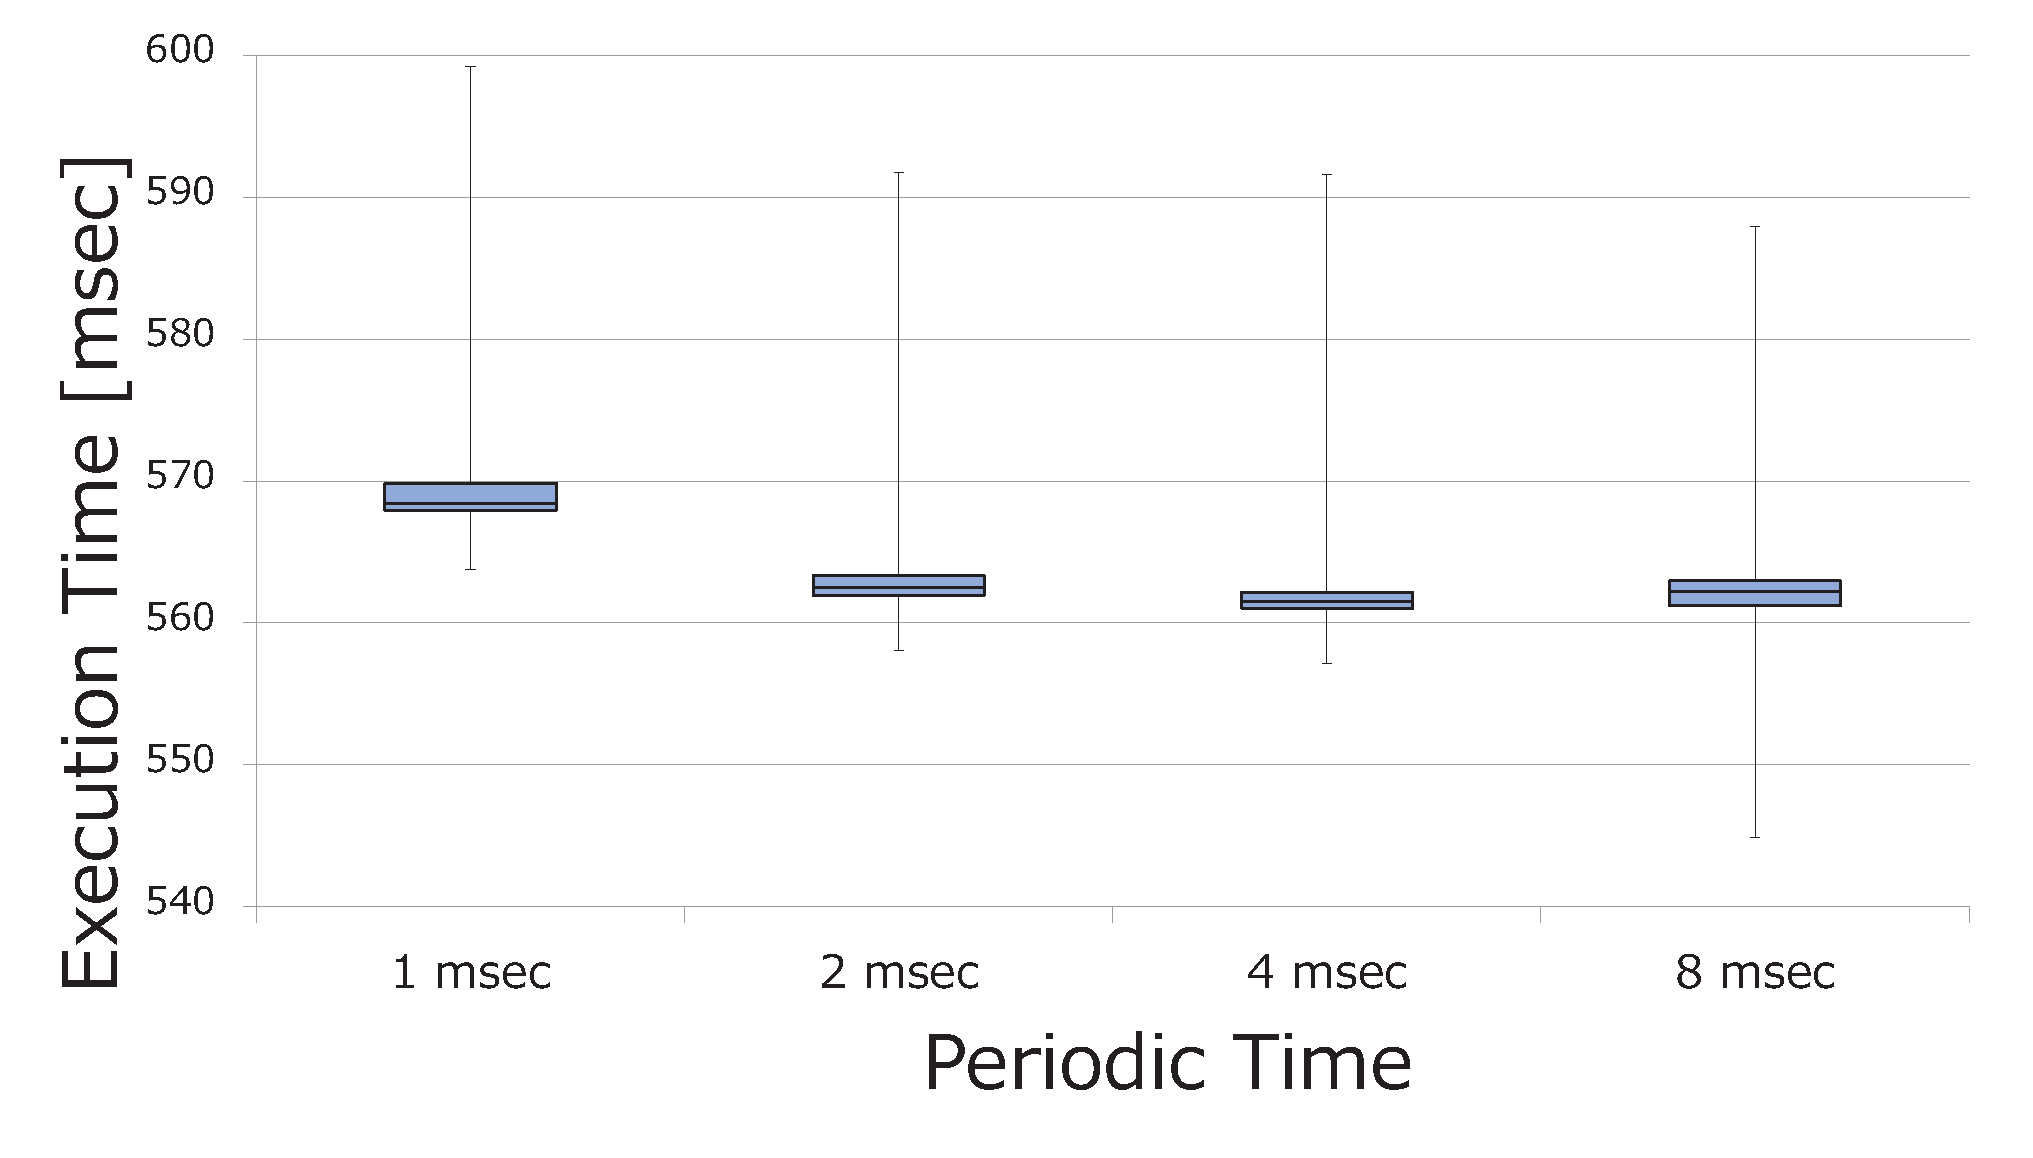
\includegraphics[width=6.5cm,clip]{figure/comparison_msec.eps}
\caption{Comparison of overhead for each cyclic period of RiteVM scheduler}
\label{fig:comparison_msec}
\end{figure}


\subsection{Synchronization of Multiple RiteVM Tasks}

 \begin{figure}[t]
    \centering
    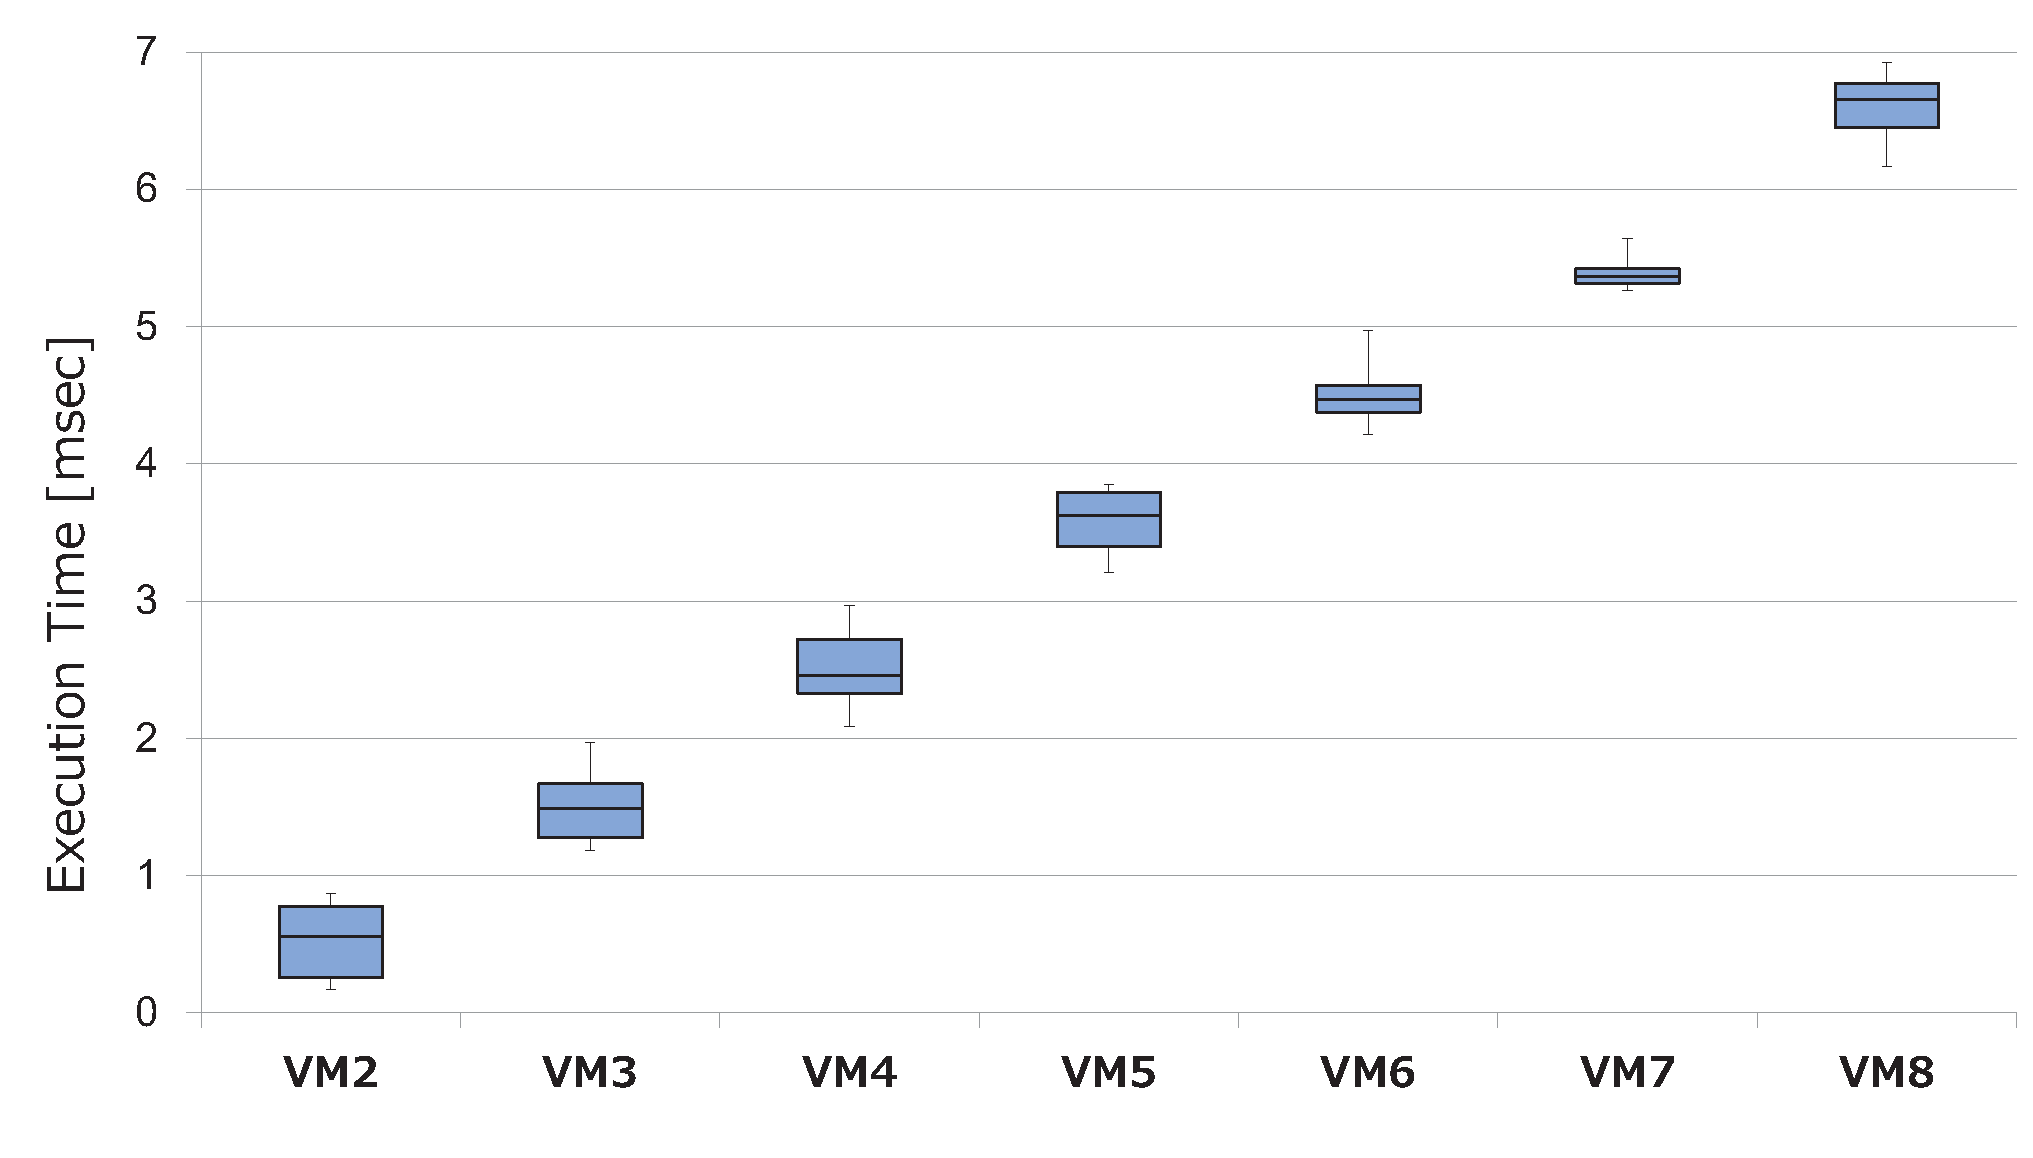
\includegraphics[width=6.5cm,clip]{figure/eval_synchronization.eps}
\caption{Synchronization of multiple RiteVM tasks}
\label{fig:eval_synchronization}
\end{figure}

To execute multiple mruby applications, a synchronization mechanism for RiteVM tasks is implemented in the proposed framework.
We measured the time from the execution of the first RiteVM task to that of the last RiteVM task.
It was confirmed that the time was within the theoretical value. Theoretical value is 
\begin{displaymath}
    {\scriptsize periodic\ time \times (number\ of\ RiteVM\ tasks - 1).}
\end{displaymath}
Fig.\ref{fig:eval_synchronization} shows the case of two to eight RiteVM tasks.
% Fig.\ref{fig:eval_synchronization} shows the case of four RiteVM tasks.
% The periodic time is one msec, and the number of RiteVM is four.
Note that the periodic time is 1 msec.
As shown in Fig.\ref{fig:eval_synchronization}, the time is within the theoretical value, which indicates successful synchronization of multiple RiteVM tasks.




\subsection{Benefits of Component-Based Development}

\begin{table}[t]
    \centering
    \caption{C and CDL file code for the number of RiteVMs}
    \footnotesize
    {\tabcolsep=0.1cm
    \begin{tabular}{c||c|c|c}
                       & (A)       & (B)     & Diff  \\ \hline
        C (Total)          & 8$\times$$\alpha$$+$134  & 130     & 8$\times$$\alpha+$4\\
        C (Modification)   & 10$\times\alpha$$-$2 & 0   &  10$\times\alpha$$-$2 \\
        CDL    & 18$\times$$\alpha$$+$25   & 18$\times$$\alpha$$+$25 & 0     \\
        \multicolumn{3}{l}{ $\alpha$ : the number of RiteVMs}
    \end{tabular}
    }
    \label{tab:codesize}
\end{table}

In the proposed framework, RiteVMs, the RiteVM scheduler, and Eventflags are implemented as TECS components.
Developers can add or remove the functionalities easily by modifying the CDL file.
Moreover, CBD decreases code size and improves productivity and maintainability.

%\subsubsection{Code size utilizing component-based development}
To demonstrate the superiority of CBD, a comparison of the number of lines of codes C and ACL codes between two situations is shown in Table \ref{tab:codesize}.
In Table \ref{tab:codesize}, (A) and (B) represent the source files in the upper and lower parts of Fig.\ref{fig:Eventflag}, respectively. 
For C, (B)'s code lines do not increase even if the number of RiteVMs increases, while (A)'s code lines increase as the number of RiteVMs increases.
Note that (B)'s C file can be utilized without modification regardless of the number of RiteVMs.
Moreover, the number of code lines of two CDL files are equal.
Skillful CBD yields advantages such as the decreased number of lines of codes and non-modified codes, which facilitates high productivity and maintainability.

\section{Related Work}
\label{sec:Related work}

\begin{table*}[t]
    \caption{Comparison of proposed and previous methods}
    \label{tab:comparison}
    \begin{center}
    {\tabcolsep=0.05cm
    \begin{tabular}{c||c|cccccc}
        & \shortstack{Bluetooth\\Loader}
        & \shortstack{Call\\C Function} 
        & \shortstack{Legacy Code of\\Embedded System} 
        & \shortstack{VM\\Management} 
        & \shortstack{VM\\Scheduler} 
        & \shortstack{Synchronization\\of Applications} \\ \hline
        python-on-a-chip \cite{url:python-on-a-chip} &            &            &            &            &             &            \\
        Owl system \cite{par:owl}                    &            & \checkmark & Partially  &            &             &            \\
        eLua \cite{url:eLua}                         &            & \checkmark & Partially  &            &             &            \\
        ChaiScript \cite{url:ChaiScript}             &            &            &            &    -       &    -        &            \\
        Squirrel \cite{url:Squirrel}                 &            & \checkmark &            &            &             &            \\
        mruby \cite{par:mruby}                       &            & \checkmark &            &            &             &            \\
        mruby on TECS \cite{par:mrubyonTECS}         &            & \checkmark & \checkmark & \checkmark &             &            \\
        Proposed framework                           & \checkmark & \checkmark & \checkmark & \checkmark & \checkmark  & \checkmark \\
    \end{tabular}
    }
    \end{center}
\end{table*}

Open-source runtime systems for scripting languages have been proposed previously such python-on-a-chip \cite{url:python-on-a-chip}, the Owl system \cite{par:owl}, eLua \cite{url:eLua}, ChaiScript\cite{url:ChaiScript}, Squirrel \cite{url:Squirrel}, mruby \cite{par:mruby}, \cite{url:mruby}, and mruby on TECS \cite{par:mrubyonTECS}.

{\bf python-on-a-chip:} python-on-a-chip (p14p) is a Python runtime system that uses a reduced Python VM called PyMite.
The VM runs a significant subset of the Python language with few resources on a microcontroller.
p14p can also run multiple stackless green threads.

{\bf Owl system:} The Owl system is an embedded Python runtime system.
It is a complete system for ARM Cortex-M3 microcontrollers.
The Owl toolchain produces relocatable memory images that are directly runnable on the microcontroller from Python code objects.
Note that the Owl system interpreter is the same as that of python-on-a-chip.

{\bf eLua:} eLua (embedded Lua) offers a full implementation of the Lua programming language for embedded systems.
Lua is one of the most popular scripting languages for embedded systems \cite{url:Lua}, \cite{par:Lua}.
Lua supports a co-routine, which is referred to as cooperative multitasking.
A co-routine in Lua is used as an independently executed thread.
Note that a co-routine can only suspend and resume multiple routines; thus, a Lua co-routine is not like multitasks in multitask systems.

{\bf ChaiScript:} ChaiScript is a scripting language to be embedded in C++ applications.
It is a dialect of ECMAScript (a.k.a. JavaScript).
ChaiScript is header only, that is, it only needs to include the header files in order to be used it in an application.
ChaiScript will support co-routines, but not now. 

{\bf Squirrel:} Squirrel is an object-oriented programming language designed as a lightweight scripting language that satisfies the real-time requirements of applications.
Squirrel was inspired by Lua.
The Squirrel API is very similar to Lua and the table code is based on that of Lua; Squirrel also supports co-routines.

{\bf mruby:} mruby, a lightweight implementation of the Ruby language, has been proposed for embedded systems.
mruby programs can run on a RiteVM, which is the VM for mruby and reads the mruby bytecode.
Note that the RiteVM only supports a single thread.
In addition, mruby supports co-routines but does not support multitasking for RTOSs.

{\bf mruby on TECS:} mruby on TECS is a component-based framework for running mruby programs.
mruby programs on TECS can be executed approximately 100 times faster than standard mruby programs.
In addition, software can be developed using CBD with mruby on TECS.
Although multitasking has been supported in the current mruby on TECS, developers must be familiar with the functions of the RTOS to use multitasking.
Co-routines are also supported by mruby on TECS.

Table \ref{tab:comparison} compares the proposed framework to previous methods.
The proposed framework implements all of the features shown in the table.
In particular, the proposed framework supports the loader, the VM scheduler, and application synchronization.
Note that the idea that a bytecode is transferred to the target device via Bluetooth can be applied to scripting languages other than mruby if the VM mechanism is used.
 
\section{Actual Results}
\label{sec:Results}
The proposed framework on LEGO MINDSTORMS EV3 \cite{url:download} has been certified for the official platform of ET Robocon 2016\footnote{http://www.etrobo.jp/2016/ (in Japanese)}.
In ET Robocon 2016, the team with the proposed framework stood second in a regional competition.

In addition, the proposed framework on LEGO MINDSTORMS EV3 has been commercialized for education by Afrel Co., Ltd\footnote{http://www.afrel.co.jp/lineup/textset (in Japanese)}, which is an official partner of LEGO Education.

\section{Conclusion}
\label{sec:Conclusion}
This paper presented an extended framework of mruby on TECS.
In the proposed framework, we implement a Bluetooth loader for mruby bytecode, a RiteVM scheduler, and synchronization mechanism.
The Bluetooth loader improves the software development efficiency because of omitting the process to rewrite a storage/ROM device and restart an RTOS on the target device.
The loader can use both Bluetooth and a wired serial connection, thus the proposed framework can be applied to various embedded systems.
The RiteVM scheduler makes multitasking more user-friendly compared to the current mruby on TECS.
Our experimental results show the advantages of the proposed framework.
The Bluetooth loader can improve the software development efficiency of mruby on TECS, and the RiteVM scheduler is effective in terms of execution time and ease of use compared to singletasking and co-routines.
In addition, synchronization of multiple RiteVM tasks is implemented in the proposed framework.

The proposed framework is developed using CBD.
In addition, the RiteVMs, RiteVM scheduler, and Eventflags are implemented as components; therefore, developers can add, remove, or reuse their functionalities easily as required.
Moreover, developers can choose fair scheduling or fixed-priority scheduling because the RiteVM scheduler can be added and removed easily.
For software developed with fixed-priority-based scheduling, developers only have to remove the RiteVM scheduler.
% Component-based development can increase productivity.
Note that our prototype system and the application programs used in the performance evaluation are all open-source and can be downloaded from our website \cite{url:download}.

In the future, CDL files for the RiteVM and mruby-TECS bridge will be generated automatically using a plugin, and developers will be able to transfer bytecodes using the ZMODEM protocol on the command line.
Moreover, we will support mruby libraries as mrbgems, which is an mruby distribution packaging system.

%%%%%%%%%%%% Acknowledgement %%%%%%%%%%%%%%%%%%%%%%%%%%%%%%%%%%%%%%%%
\section{Acknowledgement}

This work was supported by JSPS KAKENHI Grant Number 15H05305.
We would like to thank Takuya Ishikawa, Hiroshi Mimaki, and Kazuaki Tanaka for supporting this research.

%%%%%%%%%%%% Reference %%%%%%%%%%%%%%%%%%%%%%%%%%%%%%%%%%%%%%%%%%%%%%
\bibliographystyle{abbrv}
\bibliography{ref}



%%%%%%%%%%%本文終わり%%%%%%%%%%%%%%%%%%%%%%

% \begin{choshashoukai}
%
% \chosha{山本拓朗}
% {2016年大阪大学基礎工学部システム科学科卒.
% }
% \chosha{大山博司}
% {
% }
% \chosha{安積卓也}
% {
% }
%
% \end{choshashoukai}

\end{document}
